

\begin{frame}
\frametitle{Quantum theory of radiation by nonstationary systems 
        with application to high-order harmonic generation
        (Phys. Rev. A 101, 013410 (2020))}
        \framesubtitle{Convergence region for $\phi_\omega$ in $x$,
          $T=5\tau$, with $F_0=0.03\,\rm a.u.$ and $\omega_0=.114\,\rm a.u.$}
\small
\begin{textblock*}{500pt}(5pt,60pt)
%\centering
%\rotatebox{90}{
 \begin{minipage}{0.0\linewidth}
 \begin{figure}[tp]
 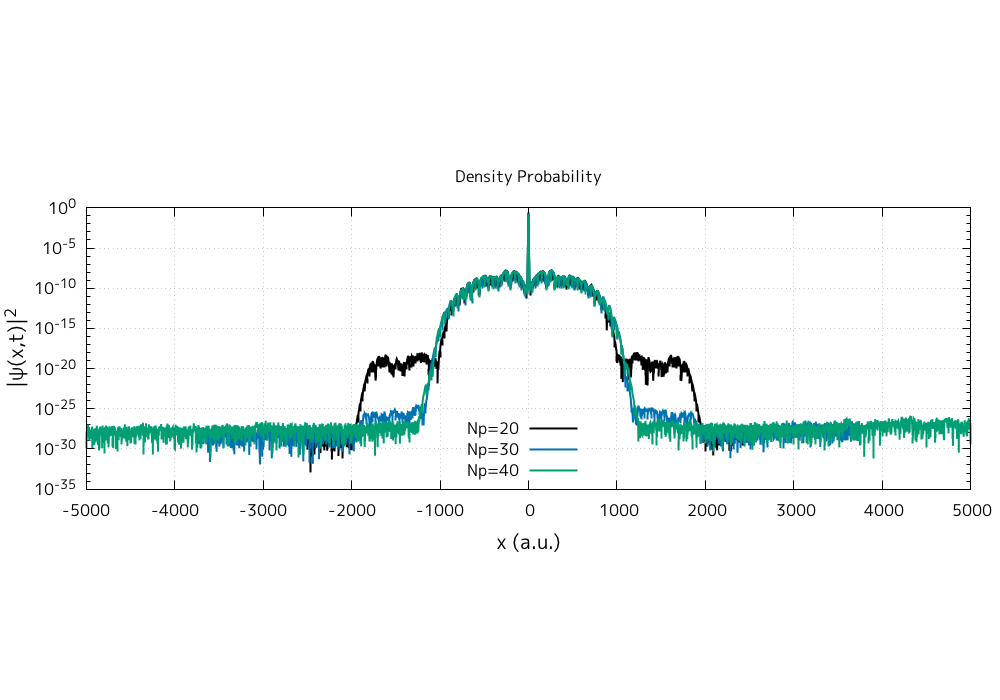
\includegraphics[scale=.18, trim={6 180 10 185},clip]{images/psi_comp_file_npns_1q4_np20_30_40.png} \\
 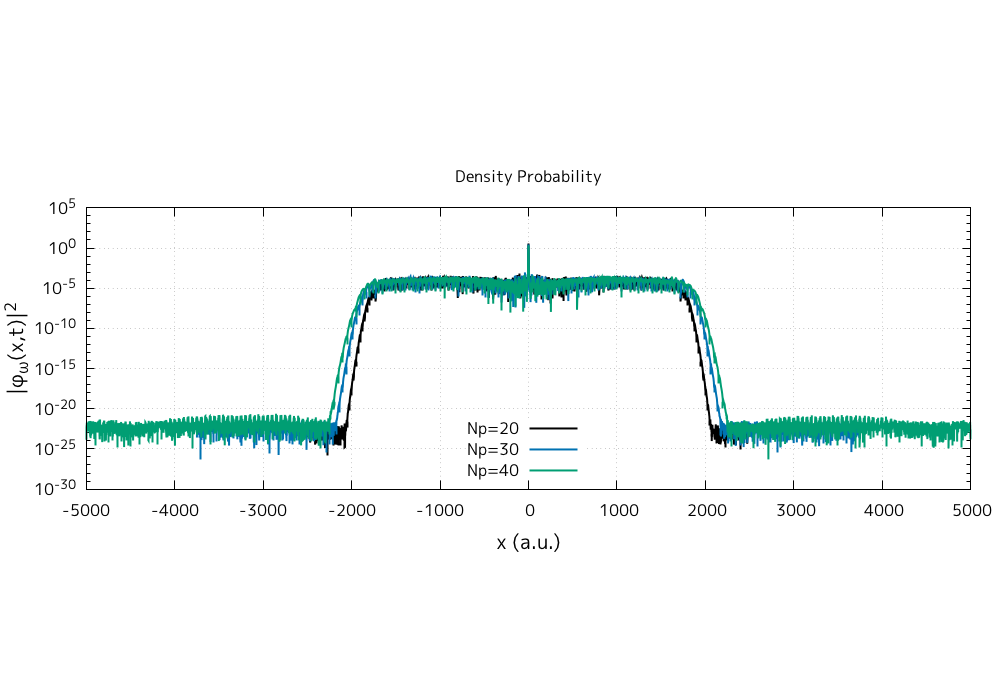
\includegraphics[scale=.18, trim={6 150 10 185},clip]{images/phi_comp_file_npns_1q4_np20_30_40.png} \\
% \includegraphics[scale=.18, trim={6 140 10 185},clip]{/s/fred/ドキュメント/電通大/hpc_fedvr_main_ref/data/exp/png_density/density_003_114_20k_25_30_200_2.png} 
%%\caption{Eigenvalues.}
%\label{fig:pemd_0114}
 \end{figure}

\end{minipage}
\end{textblock*}


\begin{textblock*}{500pt}(190pt,60pt)
%\centering
%\rotatebox{90}{
 \begin{minipage}{0.0\linewidth}
 \begin{figure}[tp]
 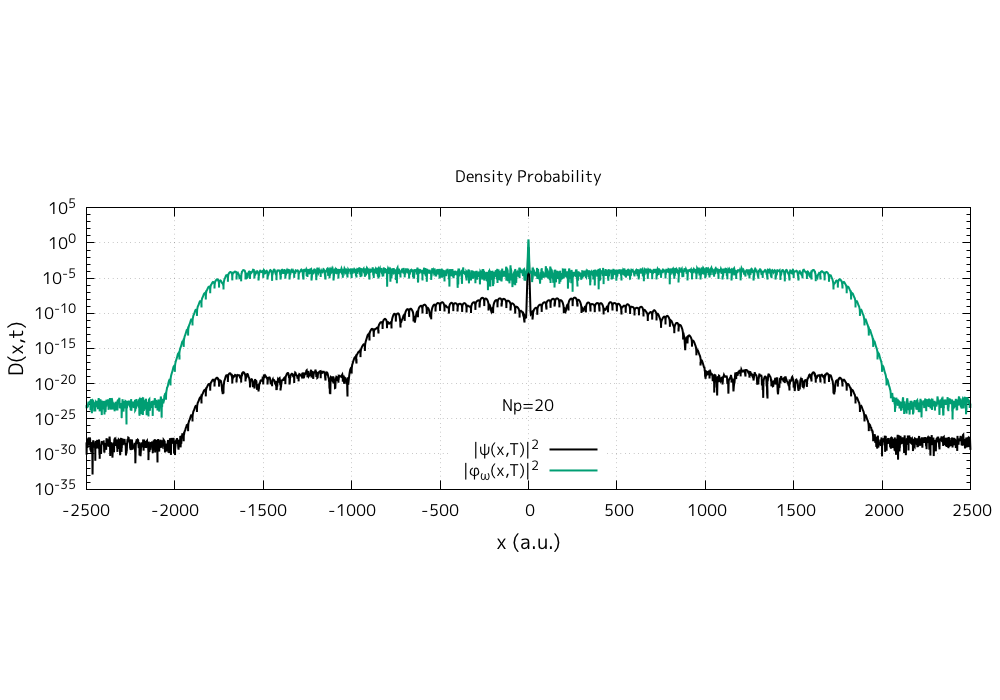
\includegraphics[scale=.18, trim={6 180 10 185},clip]{images/density_comp_file_1q4_np20.png} \\
 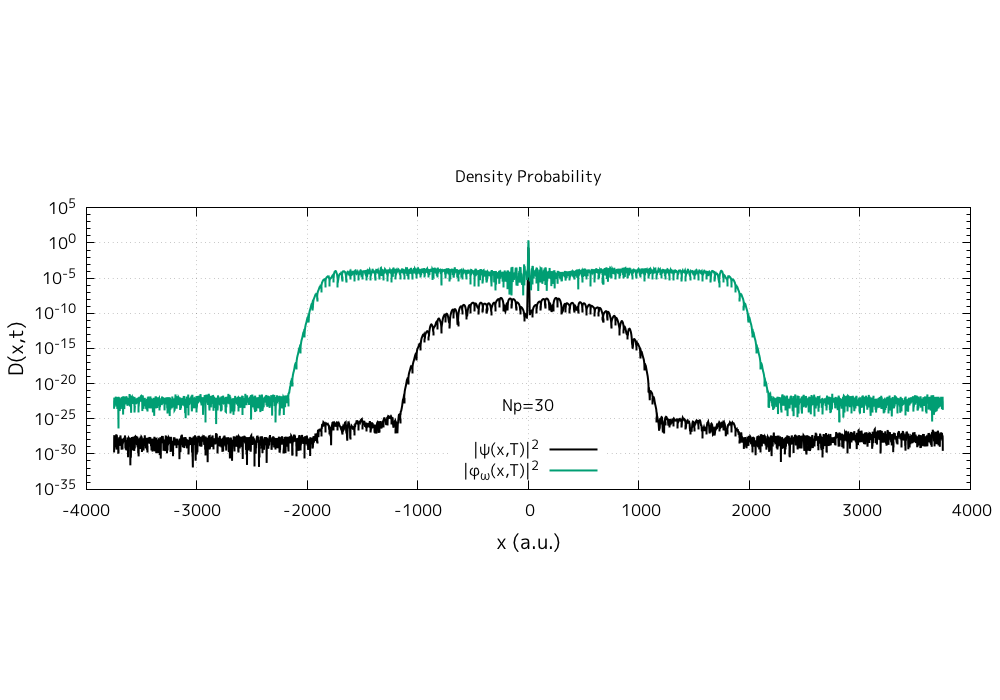
\includegraphics[scale=.18, trim={6 150 10 185},clip]{images/density_comp_file_1q4_np30.png} \\
% 
\includegraphics[scale=.20, trim={30 130 10 130},clip]{images/114_f003_12_07_hhg.png} 
%%\caption{Eigenvalues.}
%\label{fig:pemd_0114}
 \end{figure}

\end{minipage}
\end{textblock*}


%\begin{textblock*}{500pt}(390pt,165pt)
%%\centering
%\rotatebox{90}{
% \begin{minipage}{0.0\linewidth}
% \begin{figure}[tp]
% 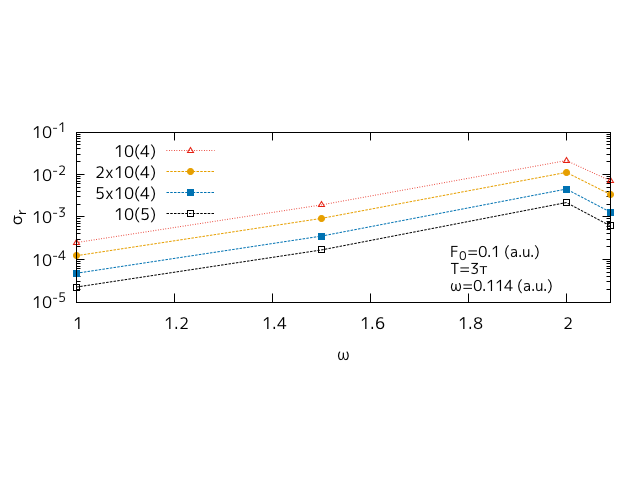
\includegraphics[scale=.20, trim={6 100 10 120},clip]{images/114_f01_3_error.png } \\
%%%\caption{Eigenvalues.}
%%\label{fig:pemd_0114}
% \end{figure}
%\end{minipage}
%}
%}
%\end{textblock*}
%
%

\begin{textblock*}{200pt}(280pt,160pt)
\rotatebox{0}{
\begin{minipage}{\linewidth}
{
\scriptsize
\centering
        \begin{align}
%               \rm{Np} = 20,\;\;\;\rm{Ns} = 100 \nonumber\\
                \;\;\;\rm{Ns} = 200 \nonumber\\
                \rm{xmax} \sim \left(\rm{Np\,Ns}+q\right)/2 \nonumber\\
                \omega_0 = 0.114\,{\rm a.u}\nonumber\\
                q=1/4\nonumber\\
                F_0 = 0.03\,{\rm a.u}, \;\;T=5\tau\nonumber\\
                {\rm nsteps} = 20 000,\, \;\;\Delta t=0.06889\nonumber
        \end{align}
%       \textcolor{red}{\textbf{The nonconvergence come from the fact that}
%       $\rm{xmax}\sim \rm{Np\,Ns}$ here}

}
\end{minipage}
}
\end{textblock*}



%\begin{textblock*}{\linewidth}(20pt,170pt)
%\rotatebox{0}{
%\begin{minipage}{\linewidth}
%{
%%\input{tables/114_f01_3t_error_2.tab}
%}
%\end{minipage}
%}
%\end{textblock*}
%
%
%\begin{textblock*}{200pt}(150pt,205pt)
%\scriptsize
%%
%\begin{align}
%	&Q^{(c)}(\omega) = \omega^2 \left| d(\omega)  \right|^2, \nonumber\\
%	&\mbox{Above is Eq.80, below is Eq.(104)} \nonumber\\
%        &Q^{(c)}(\omega) = \left| p(\omega)  \right|^2. \nonumber
%\end{align}
%
%
%\end{textblock*}


\begin{textblock*}{400pt}(30pt,200pt)
\footnotesize
\begin{itemize}
\scriptsize
\item The convergence region for $\psi$ is ${\rm xrange} \sim 2000$
\item The convergence region for $\phi$ is ${\rm xrange} \sim 4500$
\item The plateau for $\phi$ seems to be $1e-8$, 
above the double precision limit
\item The result is confirmed by 2 different methods and has been tested 
against an analytical result
\end{itemize}
\end{textblock*}


\end{frame}




\begin{frame}
\frametitle{Quantum theory of radiation by nonstationary systems 
        with application to high-order harmonic generation
        (Phys. Rev. A 101, 013410 (2020))}
        \framesubtitle{Convergence of the vector,  
         non integral transition terms $p_{k0}a_0$}
\small
\begin{textblock*}{500pt}(5pt,60pt)
%\centering
%\rotatebox{90}{
 \begin{minipage}{0.0\linewidth}
 \begin{figure}[tp]
 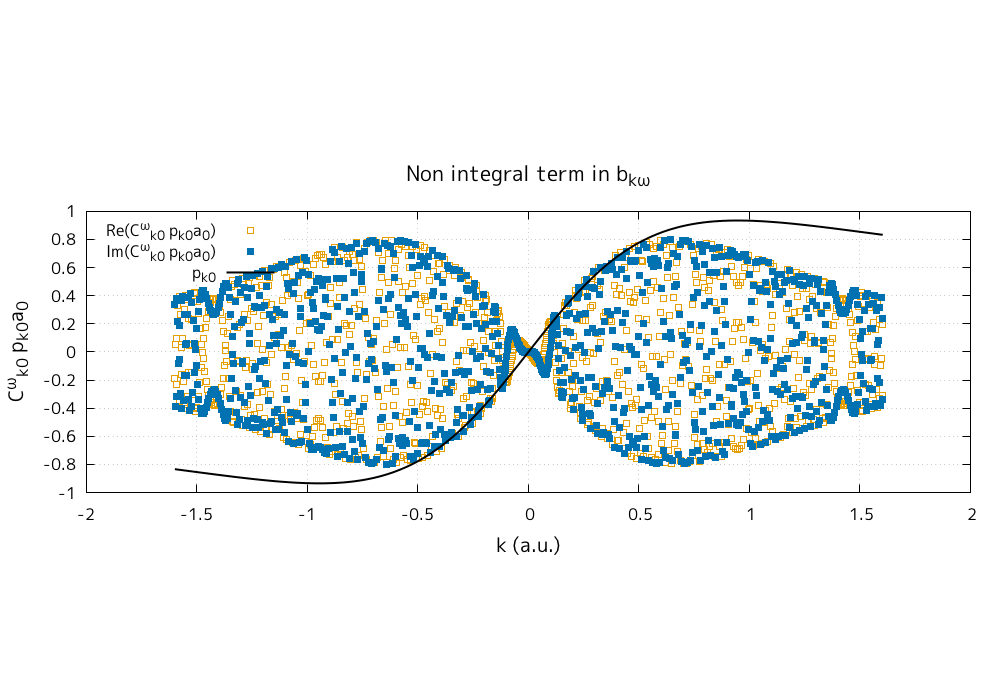
\includegraphics[scale=.18, trim={6 180 10 185},clip]{images/pk0a0_25_psi_20_200_1q10.png} \\
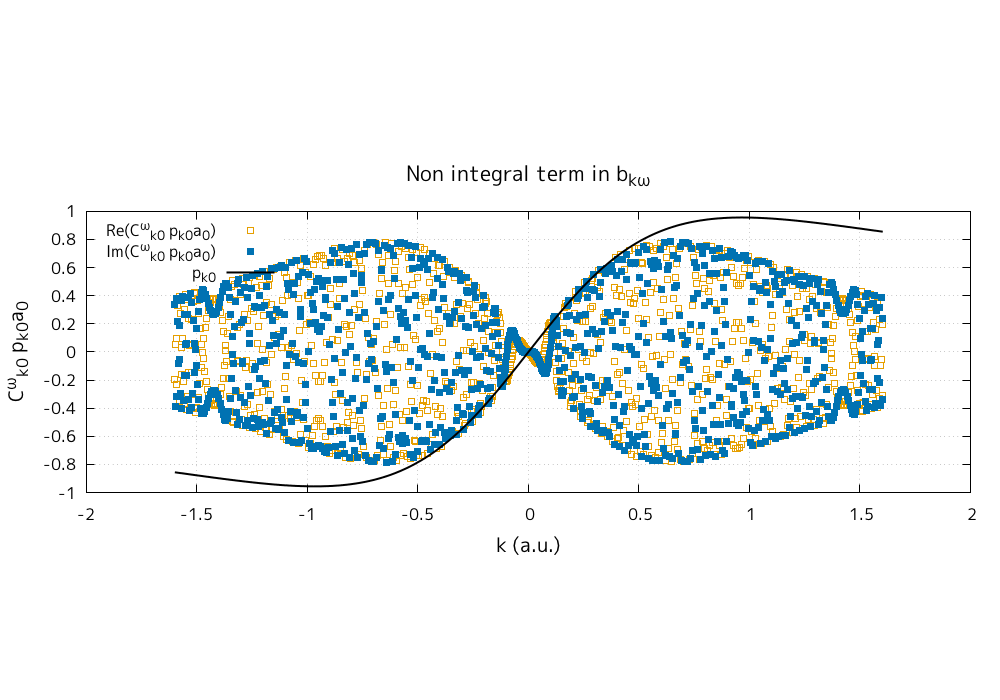
\includegraphics[scale=.18, trim={6 150 10 185},clip]{images/pk0a0_25_psi_30_200_1q10.png} \\
% \includegraphics[scale=.18, trim={6 140 10 185},clip]{/s/fred/ドキュメント/電通大/hpc_fedvr_main_ref/data/exp/png_density/density_003_114_20k_25_30_200_2.png} 
%%\caption{Eigenvalues.}
%\label{fig:pemd_0114}
 \end{figure}

\end{minipage}
\end{textblock*}


\begin{textblock*}{500pt}(190pt,60pt)
%\centering
%\rotatebox{90}{
 \begin{minipage}{0.0\linewidth}
% \begin{figure}[tp]
% 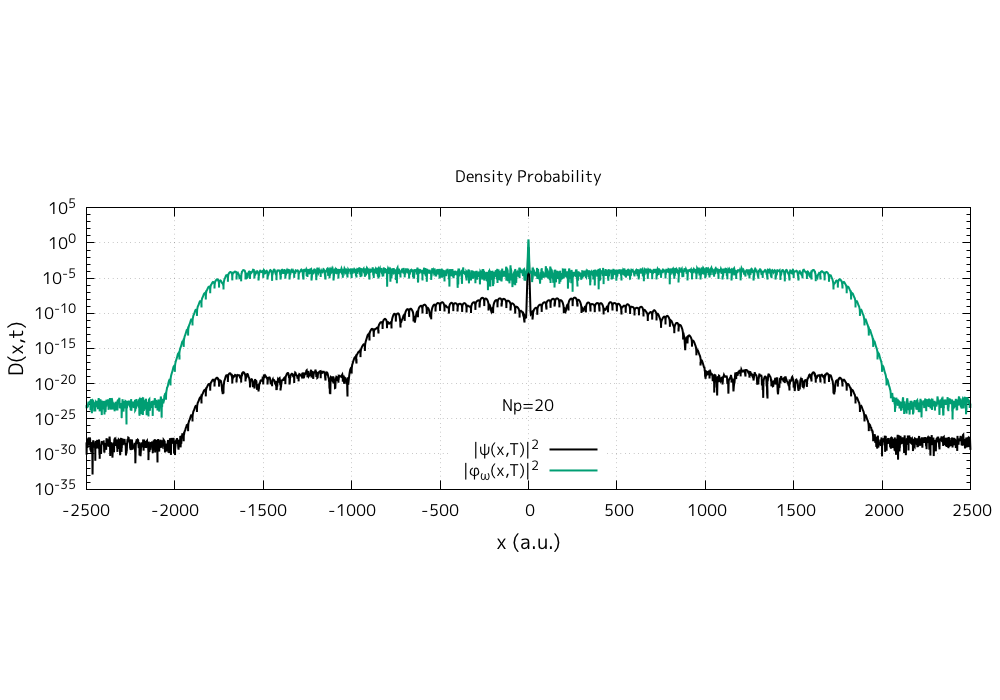
\includegraphics[scale=.18, trim={6 180 10 185},clip]{images/density_comp_file_1q4_np20.png} \\
% 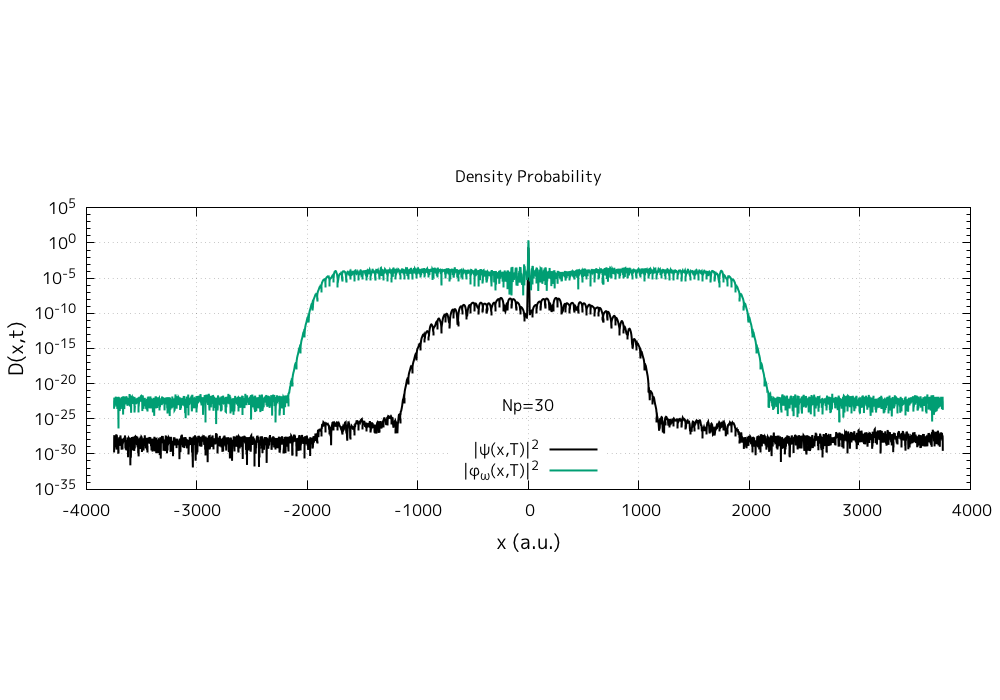
\includegraphics[scale=.18, trim={6 150 10 185},clip]{images/density_comp_file_1q4_np30.png} \\
%% 
\includegraphics[scale=.20, trim={30 130 10 130},clip]{images/114_f003_12_07_hhg.png} 
%%%\caption{Eigenvalues.}
%%\label{fig:pemd_0114}
% \end{figure}

\end{minipage}
\end{textblock*}


%\begin{textblock*}{500pt}(390pt,165pt)
%%\centering
%\rotatebox{90}{
% \begin{minipage}{0.0\linewidth}
% \begin{figure}[tp]
% 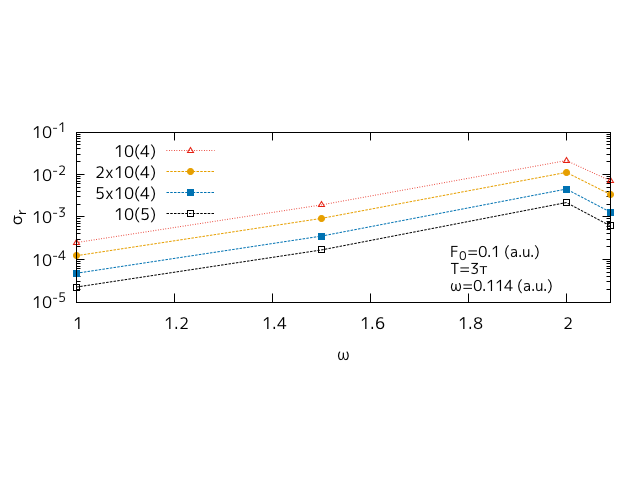
\includegraphics[scale=.20, trim={6 100 10 120},clip]{images/114_f01_3_error.png } \\
%%%\caption{Eigenvalues.}
%%\label{fig:pemd_0114}
% \end{figure}
%\end{minipage}
%}
%}
%\end{textblock*}
%
%

%\begin{textblock*}{200pt}(260pt,60pt)
\begin{textblock*}{200pt}(260pt,130pt)
\rotatebox{0}{
\begin{minipage}{\linewidth}
{
\scriptsize
\centering


%\footnotesize
%\begin{align}
%b_{0\omega}(T) & = e^{iE_0T} \int \psi_0(x) \phi_\omega(x,T) dx, \nonumber \\
%b_{k\omega}(T) & = e^{iE_kT} \int \psi_k^{(-)*}(x) \phi_\omega(x,T) dx\nonumber,
%\end{align}


\footnotesize
\begin{align}
  Q(\omega) = \left| b_{0\omega}\right|^2
        + \int \left| b_{k\omega}\right|^2 \frac{dk}{2\pi} \nonumber
\end{align}
        \begin{align}
                \rm{Np} = 20,\;\;\;\rm{Ns} = 200 \nonumber\\
%               \;\;\;\rm{Ns} = 200 \nonumber\\
                \rm{xmax} \sim \left(\rm{Np\,Ns}+q\right)/2 \nonumber\\
                \omega_0 = 0.114\,{\rm a.u}\nonumber\\
                q=1/10\nonumber\\
                F_0 = 0.03\,{\rm a.u}, \;\;T=5\tau\nonumber\\
                {\rm nsteps} = 20 000,\, \;\;\Delta t=0.06889\nonumber
        \end{align}
%       \textcolor{red}{\textbf{The nonconvergence come from the fact that}
%       $\rm{xmax}\sim \rm{Np\,Ns}$ here}

}
\end{minipage}
}
\end{textblock*}




\begin{textblock*}{100pt}(190pt,80pt)
\rotatebox{0}{
\begin{minipage}{\linewidth}
{
\scriptsize
\centering


\footnotesize
\begin{align}
  C^{\omega}_{k0} p_{k0}a_0= \frac{e^{i(E_k+\omega-E_0)T}}{E_k+\omega-E_0}
            p_{k0}a_0 \nonumber
\end{align}
}
\end{minipage}
}
\end{textblock*}



\begin{textblock*}{200pt}(30pt,190pt)
\footnotesize

\begin{align}
b_{0\omega} & = b_{0\omega}(T)
 +\int\frac{e^{i(E_0+\omega-E_{k^\prime})T}p_{0k^\prime}a_{k^\prime}}
{E_0+\omega-E_{k^\prime} + i0} \frac{dk^\prime}{2\pi} \nonumber\\
b_{k\omega} & = b_{k\omega}(T)
 +\frac{e^{i(E_k+\omega-E_0)T}p_{k0}a_0}{E_k+\omega-E_0}
 +\int\frac{e^{i(E_k+\omega-E_{k^\prime})T}p_{kk^\prime}a_{k^\prime}}
{E_k+\omega-E_{k^\prime} + i0} \frac{dk^\prime}{2\pi} \nonumber
\end{align}

%\begin{align}
% i\partial_t \phi_{\omega}(t) 
% & = \left(\hat{H}_a + \hat{V}_{\rm ext}(t) \right) \phi_{\omega}(t) \nonumber\\
% i\partial_t \phi_{\omega}(t) 
% & = \left(\hat{H}_a + \hat{V}_{\rm ext}(t) \right) \phi_{\omega}(t) 
%-i e^{i\omega t} \partial_x \psi (x,t) \nonumber
%\end{align}
%%\begin{itemize}
%\scriptsize
%\item The convergence region for $\psi$ is ${\rm xrange} \sim 2000$
%\item The convergence region for $\phi$ is ${\rm xrange} \sim 4500$
%\item The plateau for $\phi$ seems to be $1e-8$, 
%above the double precision limit
%\item The result is confirmed by 2 different methods and has been tested 
%against an analytical result
%\end{itemize}

\end{textblock*}


\end{frame}



\begin{frame}
\frametitle{Quantum theory of radiation by nonstationary systems 
        with application to high-order harmonic generation
        (Phys. Rev. A 101, 013410 (2020))}
        \framesubtitle{Convergence of the 
         integral transition terms $p_{0k^\prime}a_{k^\prime}$, and 
         $p_{kk^\prime}a_{k^\prime}$}
\small
\begin{textblock*}{500pt}(5pt,60pt)
%\centering
%\rotatebox{90}{
 \begin{minipage}{0.0\linewidth}
 \begin{figure}[tp]
 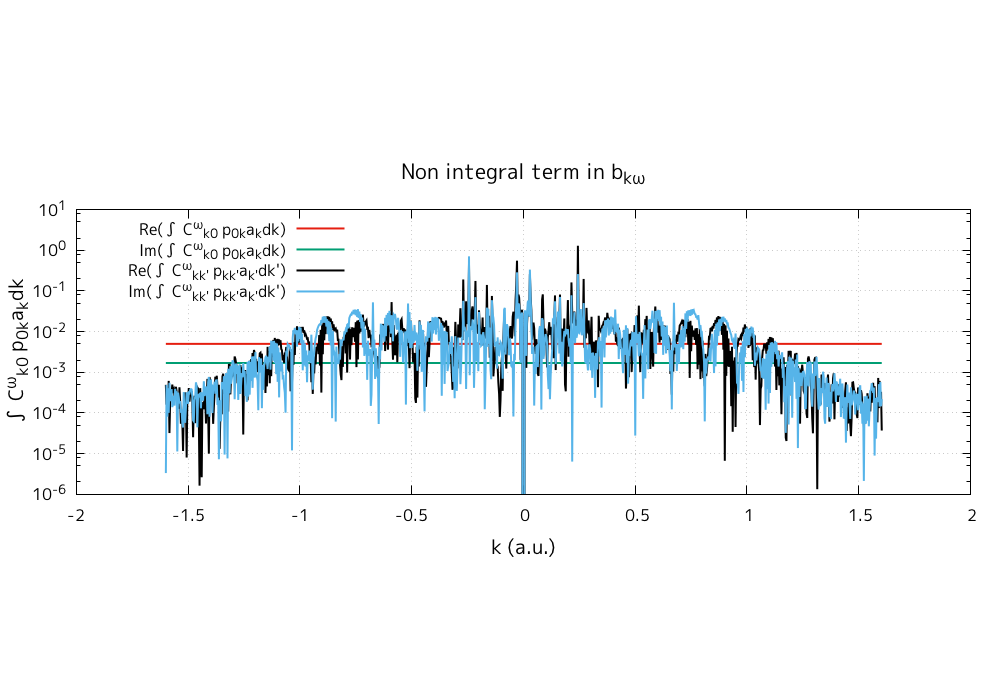
\includegraphics[scale=.18, trim={6 180 10 185},clip]{images/diff_terms_25_psi_20_200_1q10.png} \\
 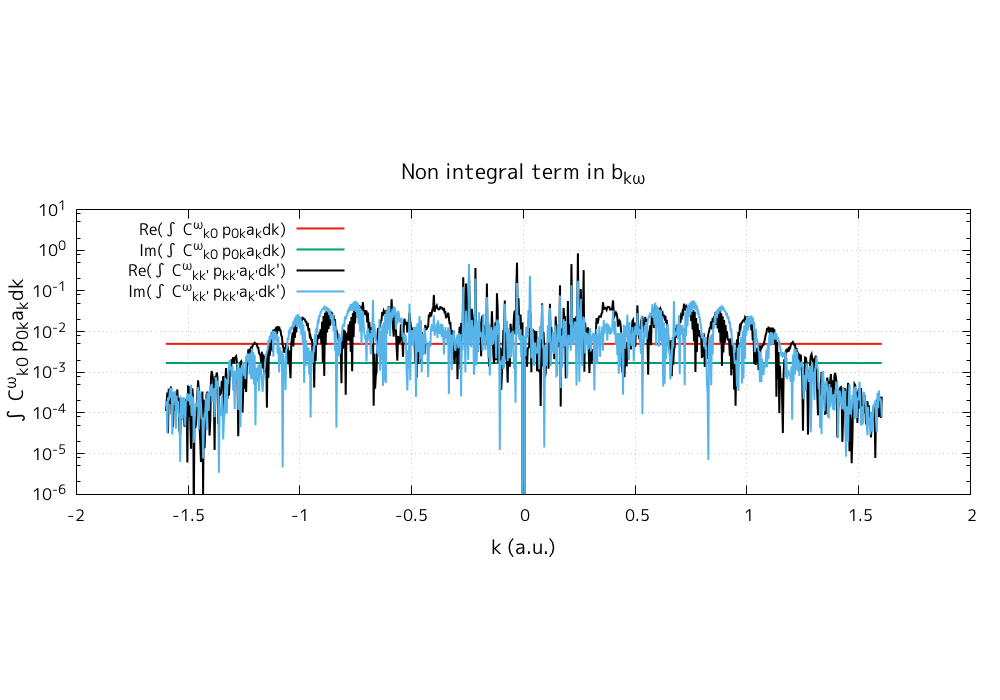
\includegraphics[scale=.18, trim={6 150 10 185},clip]{images/diff_terms_25_psi_30_200_1q10.png} \\
% \includegraphics[scale=.18, trim={6 140 10 185},clip]{/s/fred/ドキュメント/電通大/hpc_fedvr_main_ref/data/exp/png_density/density_003_114_20k_25_30_200_2.png} 
%%\caption{Eigenvalues.}
%\label{fig:pemd_0114}
 \end{figure}

\end{minipage}
\end{textblock*}


\begin{textblock*}{500pt}(190pt,60pt)
%\centering
%\rotatebox{90}{
 \begin{minipage}{0.0\linewidth}
% \begin{figure}[tp]
% 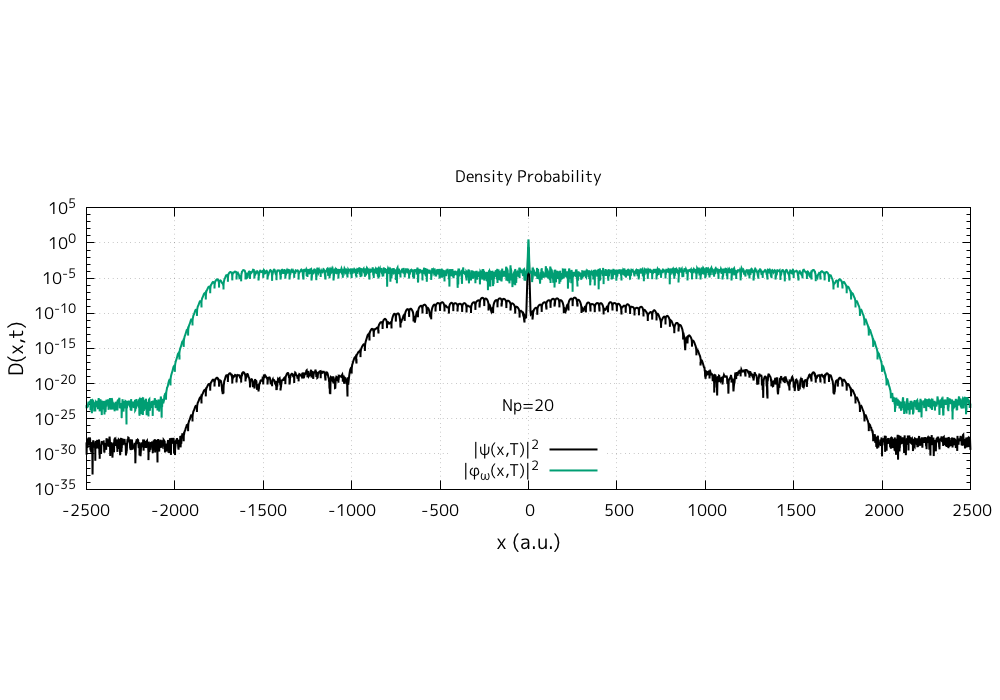
\includegraphics[scale=.18, trim={6 180 10 185},clip]{images/density_comp_file_1q4_np20.png} \\
% 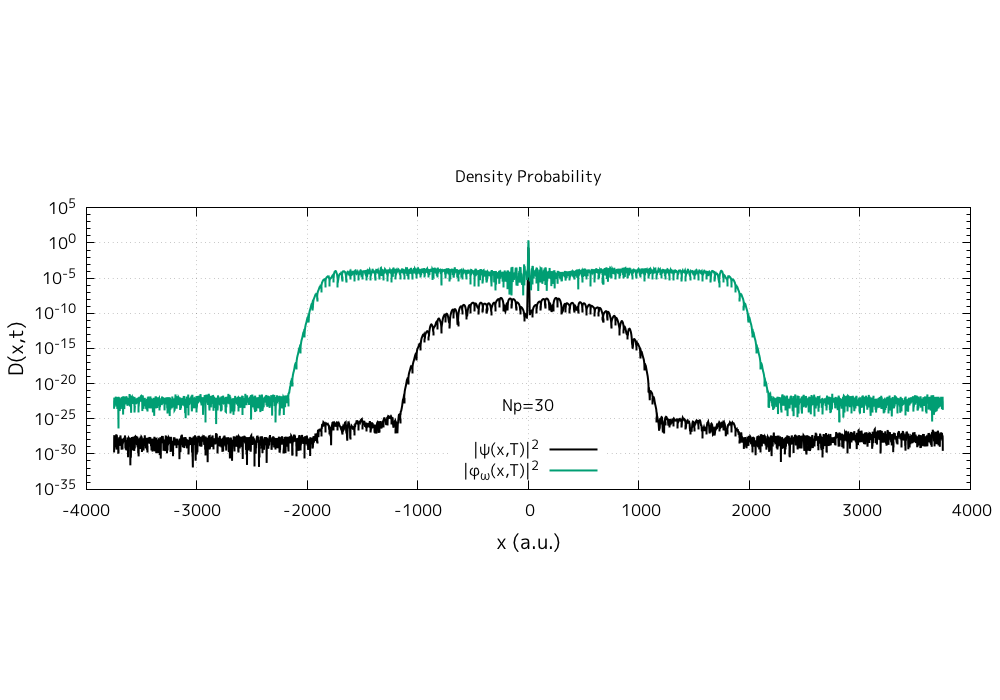
\includegraphics[scale=.18, trim={6 150 10 185},clip]{images/density_comp_file_1q4_np30.png} \\
%% 
\includegraphics[scale=.20, trim={30 130 10 130},clip]{images/114_f003_12_07_hhg.png} 
%%%\caption{Eigenvalues.}
%%\label{fig:pemd_0114}
% \end{figure}

\end{minipage}
\end{textblock*}


%\begin{textblock*}{500pt}(390pt,165pt)
%%\centering
%\rotatebox{90}{
% \begin{minipage}{0.0\linewidth}
% \begin{figure}[tp]
% 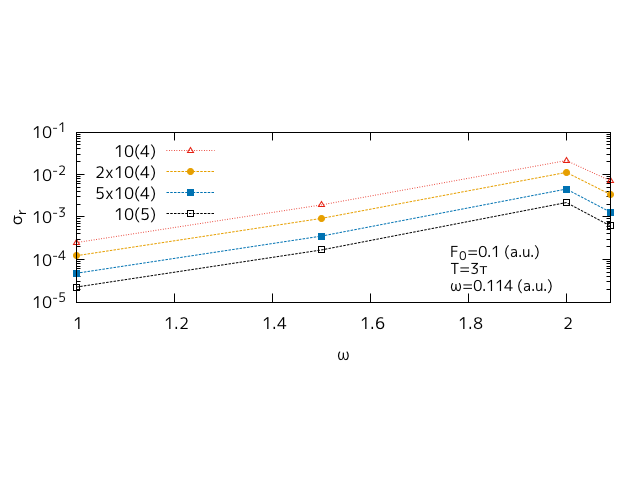
\includegraphics[scale=.20, trim={6 100 10 120},clip]{images/114_f01_3_error.png } \\
%%%\caption{Eigenvalues.}
%%\label{fig:pemd_0114}
% \end{figure}
%\end{minipage}
%}
%}
%\end{textblock*}
%
%

%\begin{textblock*}{200pt}(260pt,60pt)
\begin{textblock*}{200pt}(260pt,130pt)
\rotatebox{0}{
\begin{minipage}{\linewidth}
{
\scriptsize
\centering


\footnotesize
%\begin{align}
%b_{0\omega}(T) & = e^{iE_0T} \int \psi_0(x) \phi_\omega(x,T) dx, \nonumber \\
%b_{k\omega}(T) & = e^{iE_kT} \int \psi_k^{(-)*}(x) \phi_\omega(x,T) dx\nonumber,
%\end{align}


\footnotesize
\begin{align}
  Q(\omega) = \left| b_{0\omega}\right|^2
        + \int \left| b_{k\omega}\right|^2 \frac{dk}{2\pi} \nonumber
\end{align}
        \begin{align}
                \rm{Np} = 20,\;\;\;\rm{Ns} = 200 \nonumber\\
%               \;\;\;\rm{Ns} = 200 \nonumber\\
                \rm{xmax} \sim \left(\rm{Np\,Ns}+q\right)/2 \nonumber\\
                \omega_0 = 0.114\,{\rm a.u}\nonumber\\
                q=1/10\nonumber\\
                F_0 = 0.03\,{\rm a.u}, \;\;T=5\tau\nonumber\\
                {\rm nsteps} = 20 000,\, \;\;\Delta t=0.06889\nonumber
        \end{align}
%       \textcolor{red}{\textbf{The nonconvergence come from the fact that}
%       $\rm{xmax}\sim \rm{Np\,Ns}$ here}

}
\end{minipage}
}
\end{textblock*}




\begin{textblock*}{100pt}(190pt,80pt)
\rotatebox{0}{
\begin{minipage}{\linewidth}
{
\scriptsize
\centering


\footnotesize
\begin{align}
\int dk C^{\omega}_{0k} p_{0k}a_k & =\int  \frac{dk}{2\pi} \frac{e^{i(E_0+\omega-E_k)T}}{E_0+\omega-E_k} p_{0k}a_k\nonumber\\
\int dk^\prime C^{\omega}_{kk^\prime} p_{kk^\prime}a_{k^\prime} 
 & = \int \frac{dk^\prime}{2\pi} \frac{e^{i(E_k+\omega-E_{k^\prime})T}}{E_k+\omega-E_{k^\prime}} 
p_{kk^\prime} a_{k^\prime}    \nonumber
\end{align}
}
\end{minipage}
}
\end{textblock*}



\begin{textblock*}{200pt}(30pt,190pt)
\footnotesize

\begin{align}
b_{0\omega} & = b_{0\omega}(T)
 +\int\frac{e^{i(E_0+\omega-E_{k^\prime})T}p_{0k^\prime}a_{k^\prime}}
{E_0+\omega-E_{k^\prime} + i0} \frac{dk^\prime}{2\pi} \nonumber\\
b_{k\omega} & = b_{k\omega}(T)
 +\frac{e^{i(E_k+\omega-E_0)T}p_{k0}a_0}{E_k+\omega-E_0}
 +\int\frac{e^{i(E_k+\omega-E_{k^\prime})T}p_{kk^\prime}a_{k^\prime}}
{E_k+\omega-E_{k^\prime} + i0} \frac{dk^\prime}{2\pi} \nonumber
\end{align}

%\begin{align}
% i\partial_t \phi_{\omega}(t) 
% & = \left(\hat{H}_a + \hat{V}_{\rm ext}(t) \right) \phi_{\omega}(t) \nonumber\\
% i\partial_t \phi_{\omega}(t) 
% & = \left(\hat{H}_a + \hat{V}_{\rm ext}(t) \right) \phi_{\omega}(t) 
%-i e^{i\omega t} \partial_x \psi (x,t) \nonumber
%\end{align}
%%\begin{itemize}
%\scriptsize
%\item The convergence region for $\psi$ is ${\rm xrange} \sim 2000$
%\item The convergence region for $\phi$ is ${\rm xrange} \sim 4500$
%\item The plateau for $\phi$ seems to be $1e-8$, 
%above the double precision limit
%\item The result is confirmed by 2 different methods and has been tested 
%against an analytical result
%\end{itemize}

\end{textblock*}


\end{frame}








\begin{frame}
\frametitle{Quantum theory of radiation by nonstationary systems 
        with application to high-order harmonic generation
        (Phys. Rev. A 101, 013410 (2020))}
        \framesubtitle{Convergence of the 
         integral transition terms $p_{0k^\prime}a_{k^\prime}$, and 
         $p_{kk^\prime}a_{k^\prime}$}
\small
\begin{textblock*}{500pt}(5pt,60pt)
%\centering
%\rotatebox{90}{
 \begin{minipage}{0.0\linewidth}
 \begin{figure}[tp]
 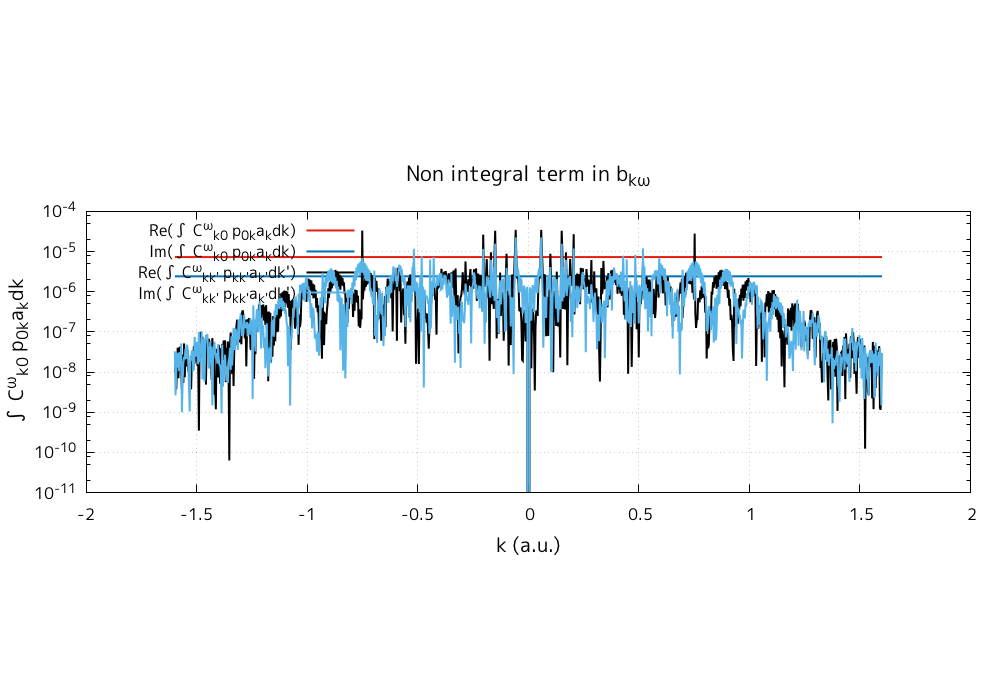
\includegraphics[scale=.18, trim={6 180 10 185},clip]{images/diff_terms_25_psi_20_200_1q10_improved.png} \\
%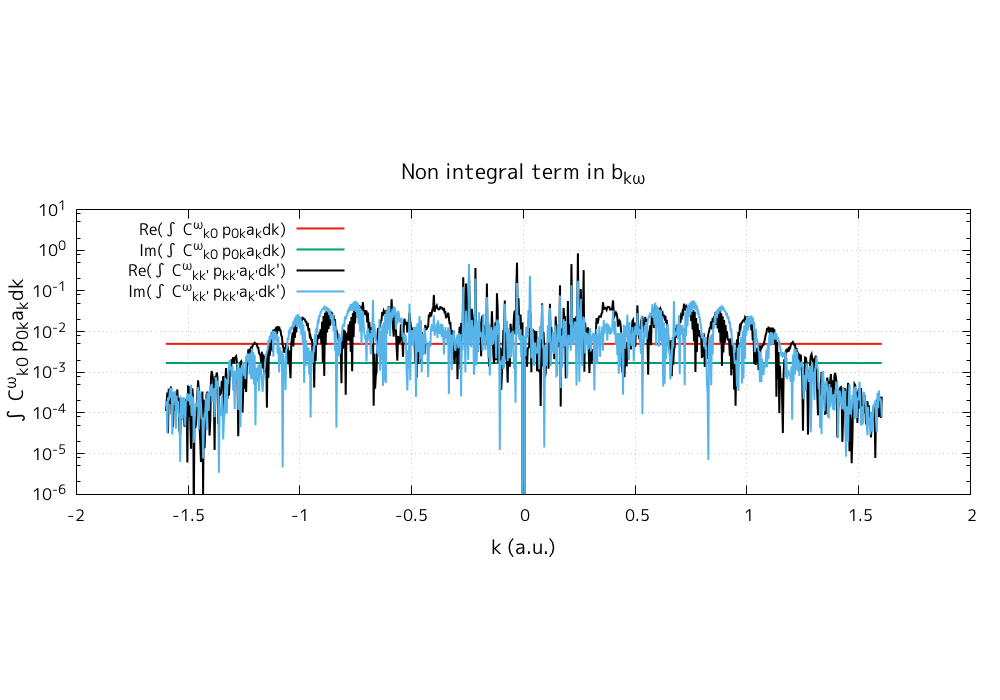
\includegraphics[scale=.18, trim={6 150 10 185},clip]{images/diff_terms_25_psi_30_200_1q10.png} \\
% \includegraphics[scale=.18, trim={6 140 10 185},clip]{/s/fred/ドキュメント/電通大/hpc_fedvr_main_ref/data/exp/png_density/density_003_114_20k_25_30_200_2.png} 
%%\caption{Eigenvalues.}
%\label{fig:pemd_0114}
 \end{figure}

\end{minipage}
\end{textblock*}


\begin{textblock*}{500pt}(190pt,60pt)
%\centering
%\rotatebox{90}{
 \begin{minipage}{0.0\linewidth}
% \begin{figure}[tp]
% 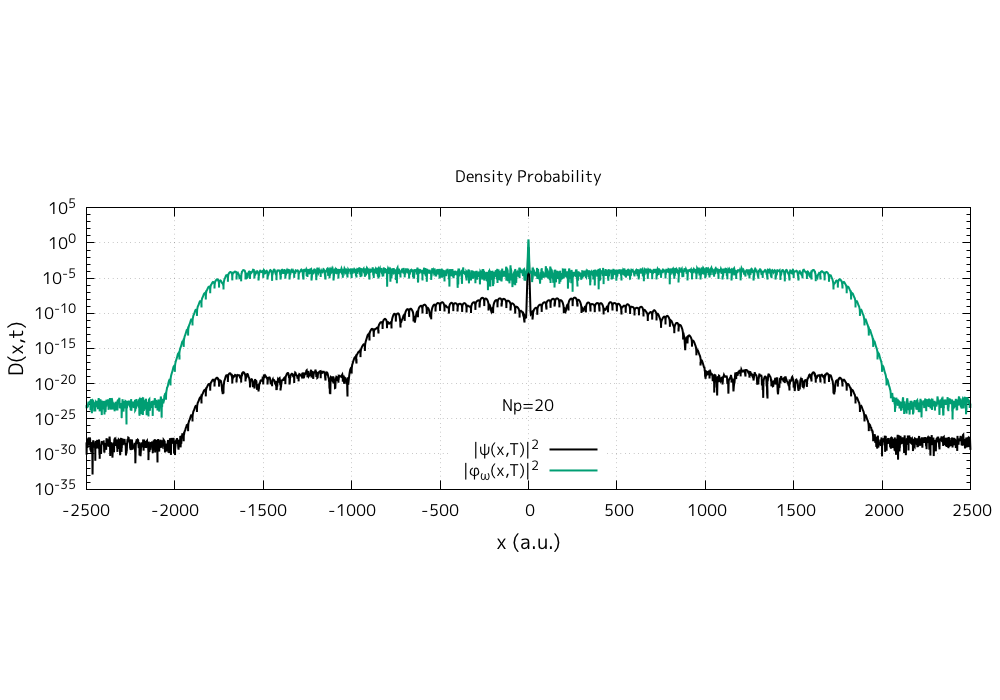
\includegraphics[scale=.18, trim={6 180 10 185},clip]{images/density_comp_file_1q4_np20.png} \\
% 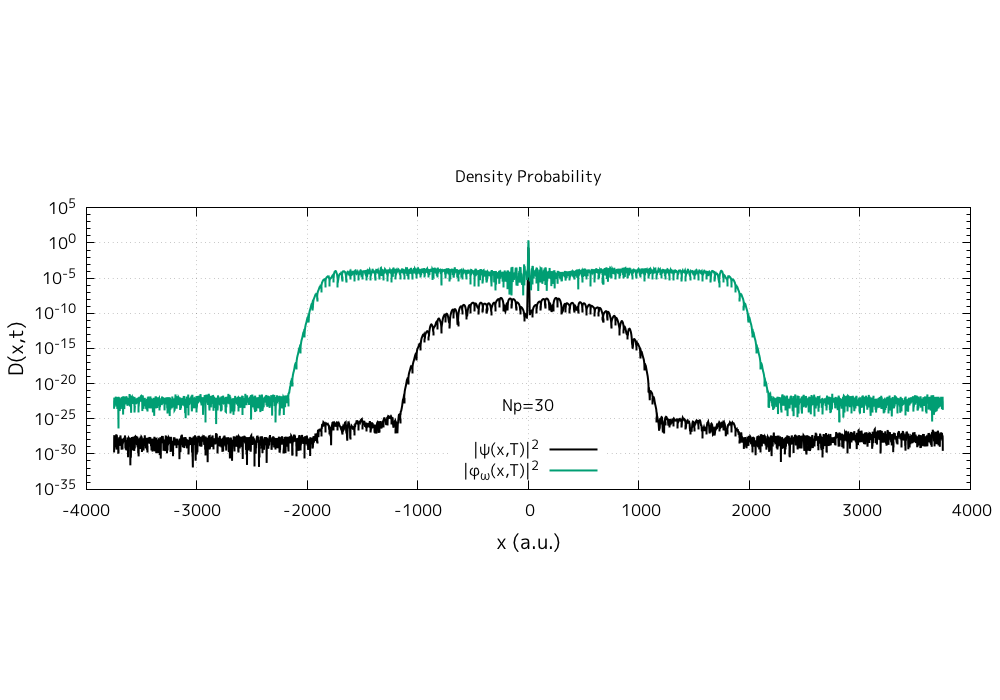
\includegraphics[scale=.18, trim={6 150 10 185},clip]{images/density_comp_file_1q4_np30.png} \\
%% 
\includegraphics[scale=.20, trim={30 130 10 130},clip]{images/114_f003_12_07_hhg.png} 
%%%\caption{Eigenvalues.}
%%\label{fig:pemd_0114}
% \end{figure}

\end{minipage}
\end{textblock*}


%\begin{textblock*}{500pt}(390pt,165pt)
%%\centering
%\rotatebox{90}{
% \begin{minipage}{0.0\linewidth}
% \begin{figure}[tp]
% 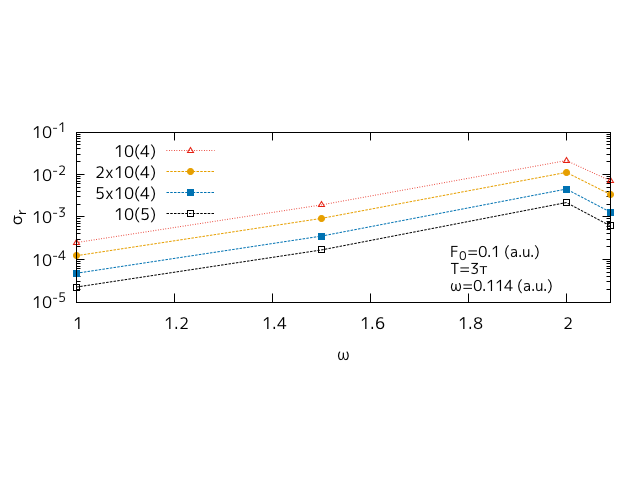
\includegraphics[scale=.20, trim={6 100 10 120},clip]{images/114_f01_3_error.png } \\
%%%\caption{Eigenvalues.}
%%\label{fig:pemd_0114}
% \end{figure}
%\end{minipage}
%}
%}
%\end{textblock*}
%
%

%\begin{textblock*}{200pt}(260pt,60pt)
\begin{textblock*}{200pt}(260pt,130pt)
\rotatebox{0}{
\begin{minipage}{\linewidth}
{
\scriptsize
\centering


\footnotesize
%\begin{align}
%b_{0\omega}(T) & = e^{iE_0T} \int \psi_0(x) \phi_\omega(x,T) dx, \nonumber \\
%b_{k\omega}(T) & = e^{iE_kT} \int \psi_k^{(-)*}(x) \phi_\omega(x,T) dx\nonumber,
%\end{align}


\footnotesize
\begin{align}
  Q(\omega) = \left| b_{0\omega}\right|^2
        + \int \left| b_{k\omega}\right|^2 \frac{dk}{2\pi} \nonumber
\end{align}
        \begin{align}
                \rm{Np} = 20,\;\;\;\rm{Ns} = 200 \nonumber\\
%               \;\;\;\rm{Ns} = 200 \nonumber\\
                \rm{xmax} \sim \left(\rm{Np\,Ns}+q\right)/2 \nonumber\\
                \omega_0 = 0.114\,{\rm a.u}\nonumber\\
                q=1/10\nonumber\\
                F_0 = 0.03\,{\rm a.u}, \;\;T=5\tau\nonumber\\
                {\rm nsteps} = 20 000,\, \;\;\Delta t=0.06889\nonumber
        \end{align}
%       \textcolor{red}{\textbf{The nonconvergence come from the fact that}
%       $\rm{xmax}\sim \rm{Np\,Ns}$ here}

}
\end{minipage}
}
\end{textblock*}




\begin{textblock*}{100pt}(190pt,80pt)
\rotatebox{0}{
\begin{minipage}{\linewidth}
{
\scriptsize
\centering


\footnotesize
\begin{align}
\int dk C^{\omega}_{0k} p_{0k}a_k & =\int  \frac{dk}{2\pi} \frac{e^{i(E_0+\omega-E_k)T}}{E_0+\omega-E_k} p_{0k}a_k\nonumber\\
\int dk^\prime C^{\omega}_{kk^\prime} p_{kk^\prime}a_{k^\prime} 
 & = \int \frac{dk^\prime}{2\pi} \frac{e^{i(E_k+\omega-E_{k^\prime})T}}{E_k+\omega-E_{k^\prime}} 
p_{kk^\prime} a_{k^\prime}    \nonumber
\end{align}
}
\end{minipage}
}
\end{textblock*}



\begin{textblock*}{200pt}(30pt,190pt)
\footnotesize

\begin{align}
b_{0\omega} & = b_{0\omega}(T)
 +\int\frac{e^{i(E_0+\omega-E_{k^\prime})T}p_{0k^\prime}a_{k^\prime}}
{E_0+\omega-E_{k^\prime} + i0} \frac{dk^\prime}{2\pi} \nonumber\\
b_{k\omega} & = b_{k\omega}(T)
 +\frac{e^{i(E_k+\omega-E_0)T}p_{k0}a_0}{E_k+\omega-E_0}
 +\int\frac{e^{i(E_k+\omega-E_{k^\prime})T}p_{kk^\prime}a_{k^\prime}}
{E_k+\omega-E_{k^\prime} + i0} \frac{dk^\prime}{2\pi} \nonumber
\end{align}

%\begin{align}
% i\partial_t \phi_{\omega}(t) 
% & = \left(\hat{H}_a + \hat{V}_{\rm ext}(t) \right) \phi_{\omega}(t) \nonumber\\
% i\partial_t \phi_{\omega}(t) 
% & = \left(\hat{H}_a + \hat{V}_{\rm ext}(t) \right) \phi_{\omega}(t) 
%-i e^{i\omega t} \partial_x \psi (x,t) \nonumber
%\end{align}
%%\begin{itemize}
%\scriptsize
%\item The convergence region for $\psi$ is ${\rm xrange} \sim 2000$
%\item The convergence region for $\phi$ is ${\rm xrange} \sim 4500$
%\item The plateau for $\phi$ seems to be $1e-8$, 
%above the double precision limit
%\item The result is confirmed by 2 different methods and has been tested 
%against an analytical result
%\end{itemize}

\end{textblock*}


\end{frame}






\begin{frame}
\frametitle{Quantum theory of radiation by nonstationary systems 
        with application to high-order harmonic generation
        (Phys. Rev. A 101, 013410 (2020))}
        \framesubtitle{Study of the the coefficients $b_{k\omega}(T)$, 
         norm and PEMD (a look back)}
\small
\begin{textblock*}{500pt}(5pt,60pt)
%\centering
%\rotatebox{90}{
 \begin{minipage}{0.0\linewidth}
 \begin{figure}[tp]
 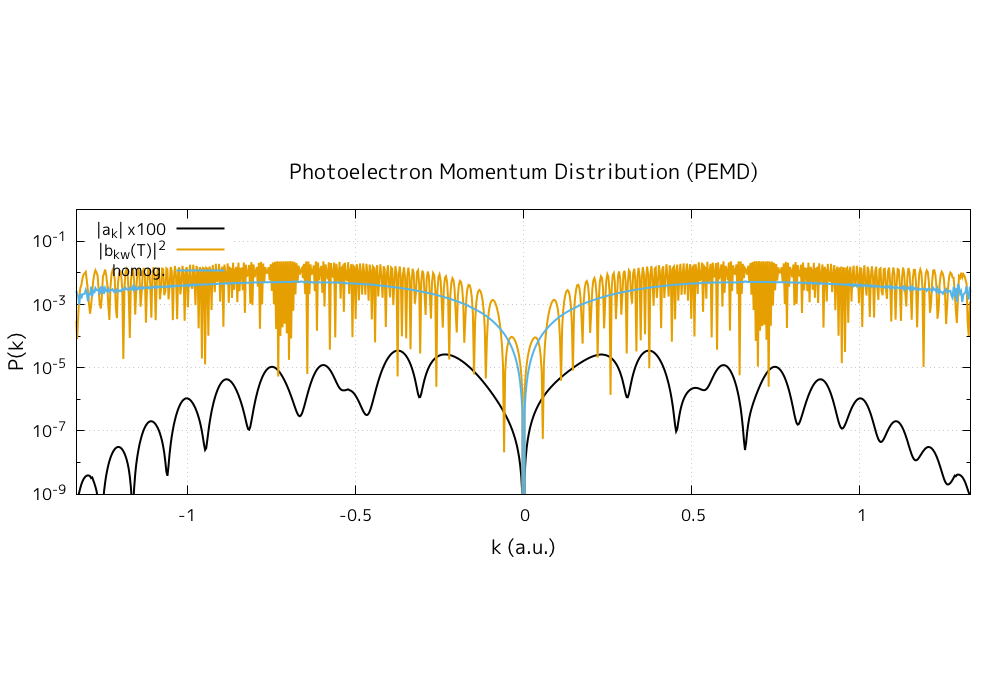
\includegraphics[scale=.18, trim={6 180 10 185},clip]{images/pemd_akbkw_20_200_1q10_k1000.png} \\
 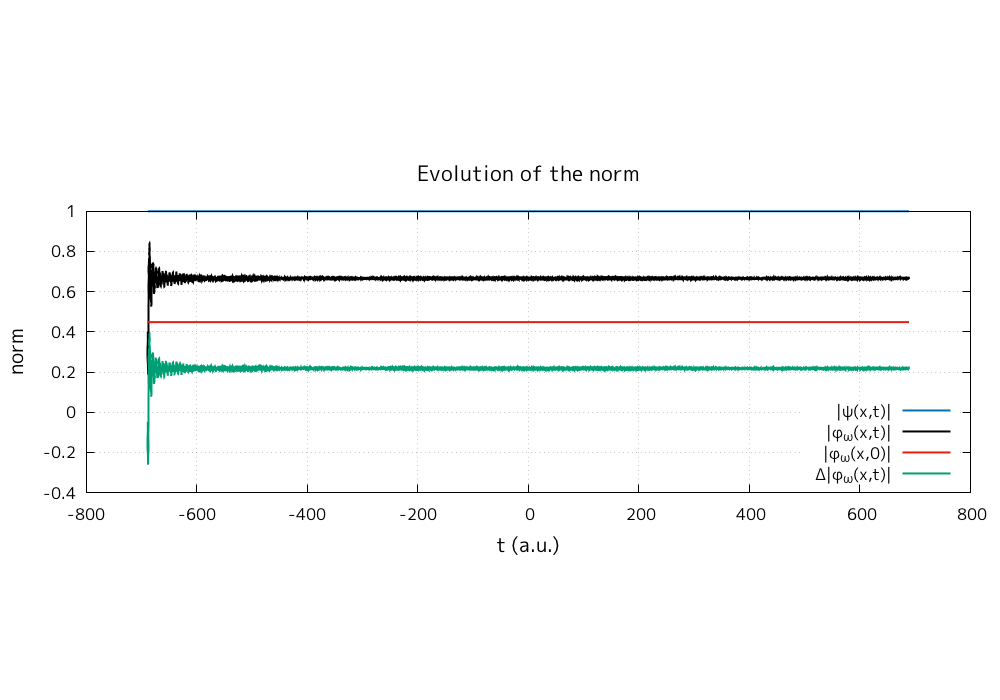
\includegraphics[scale=.18, trim={6 150 10 185},clip]{images/norm_20_200_20k_1q10.png} \\
% \includegraphics[scale=.18, trim={6 140 10 185},clip]{/s/fred/ドキュメント/電通大/hpc_fedvr_main_ref/data/exp/png_density/density_003_114_20k_25_30_200_2.png} 
%%\caption{Eigenvalues.}
%\label{fig:pemd_0114}
 \end{figure}

\end{minipage}
\end{textblock*}


\begin{textblock*}{500pt}(190pt,60pt)
%\centering
%\rotatebox{90}{
 \begin{minipage}{0.0\linewidth}
% \begin{figure}[tp]
% 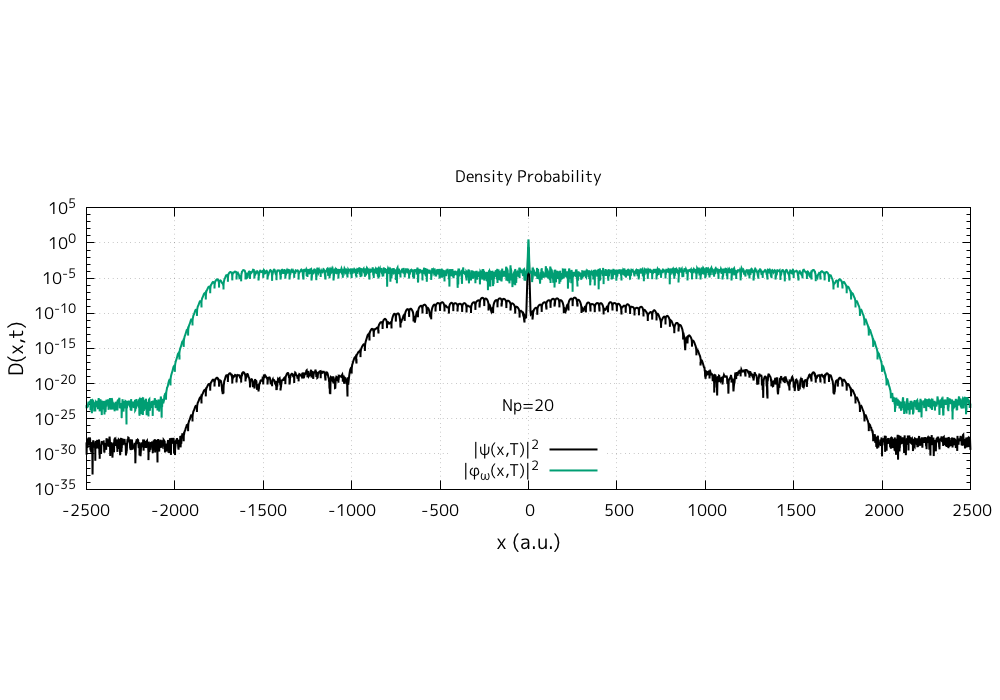
\includegraphics[scale=.18, trim={6 180 10 185},clip]{images/density_comp_file_1q4_np20.png} \\
% 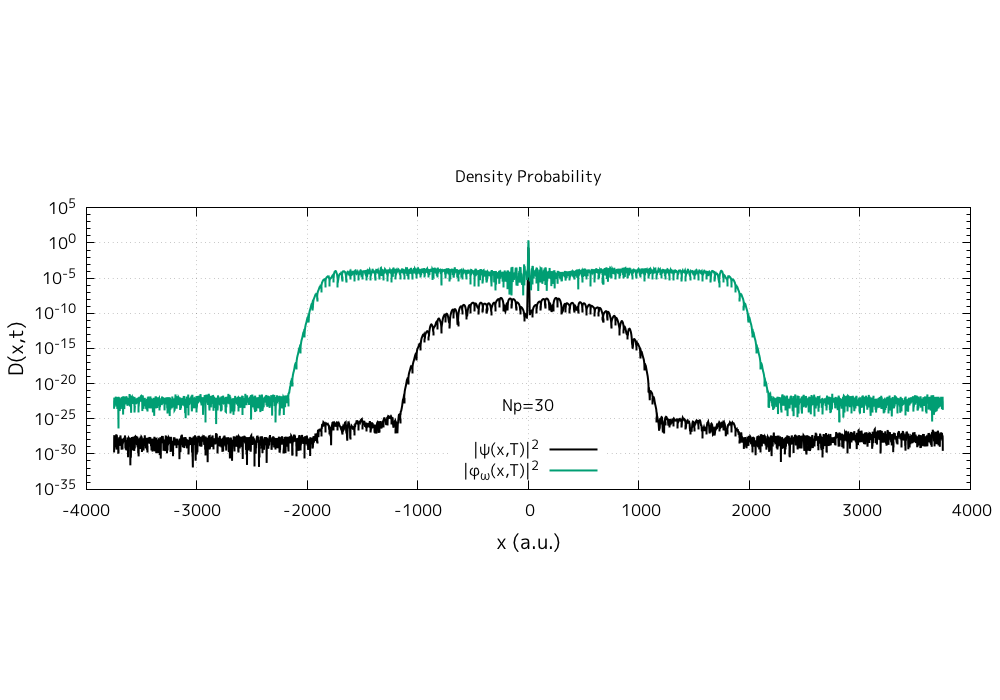
\includegraphics[scale=.18, trim={6 150 10 185},clip]{images/density_comp_file_1q4_np30.png} \\
%% 
\includegraphics[scale=.20, trim={30 130 10 130},clip]{images/114_f003_12_07_hhg.png} 
%%%\caption{Eigenvalues.}
%%\label{fig:pemd_0114}
% \end{figure}

\end{minipage}
\end{textblock*}


%

\begin{textblock*}{200pt}(260pt,130pt)
\rotatebox{0}{
\begin{minipage}{\linewidth}
{
\scriptsize
\centering


\footnotesize
\begin{align}
  Q(\omega) = \left| b_{0\omega}\right|^2
        + \int \left| b_{k\omega}\right|^2 \frac{dk}{2\pi} \nonumber
\end{align}
        \begin{align}
                \rm{Np} = 20,\;\;\;\rm{Ns} = 200 \nonumber\\
%               \;\;\;\rm{Ns} = 200 \nonumber\\
                \rm{xmax} \sim \left(\rm{Np\,Ns}+q\right)/2 \nonumber\\
                \omega_0 = 0.114\,{\rm a.u}\nonumber\\
                q=1/10\nonumber\\
                F_0 = 0.03\,{\rm a.u}, \;\;T=5\tau\nonumber\\
                {\rm nsteps} = 20 000,\, \;\;\Delta t=0.06889\nonumber
        \end{align}
%       \textcolor{red}{\textbf{The nonconvergence come from the fact that}
%       $\rm{xmax}\sim \rm{Np\,Ns}$ here}

}
\end{minipage}
}
\end{textblock*}




\begin{textblock*}{200pt}(270pt,80pt)
\rotatebox{0}{
\begin{minipage}{\linewidth}
{
\scriptsize
\centering

\footnotesize
\begin{align}
b_{0\omega}(T) & = e^{iE_0T} \int \psi_0(x) \phi_\omega(x,T) dx, \nonumber \\
b_{k\omega}(T) & = e^{iE_kT} \int \psi_k^{(-)*}(x) \phi_\omega(x,T) dx\nonumber,
\end{align}
}
\end{minipage}
}
\end{textblock*}



\begin{textblock*}{200pt}(30pt,190pt)
\footnotesize

\begin{align}
b_{0\omega} & = b_{0\omega}(T)
 +\int\frac{e^{i(E_0+\omega-E_{k^\prime})T}p_{0k^\prime}a_{k^\prime}}
{E_0+\omega-E_{k^\prime} + i0} \frac{dk^\prime}{2\pi} \nonumber\\
b_{k\omega} & = b_{k\omega}(T)
 +\frac{e^{i(E_k+\omega-E_0)T}p_{k0}a_0}{E_k+\omega-E_0}
 +\int\frac{e^{i(E_k+\omega-E_{k^\prime})T}p_{kk^\prime}a_{k^\prime}}
{E_k+\omega-E_{k^\prime} + i0} \frac{dk^\prime}{2\pi} \nonumber
\end{align}

%\begin{align}
% i\partial_t \phi_{\omega}(t) 
% & = \left(\hat{H}_a + \hat{V}_{\rm ext}(t) \right) \phi_{\omega}(t) \nonumber\\
% i\partial_t \phi_{\omega}(t) 
% & = \left(\hat{H}_a + \hat{V}_{\rm ext}(t) \right) \phi_{\omega}(t) 
%-i e^{i\omega t} \partial_x \psi (x,t) \nonumber
%\end{align}
%%\begin{itemize}
%\scriptsize
%\item The convergence region for $\psi$ is ${\rm xrange} \sim 2000$
%\item The convergence region for $\phi$ is ${\rm xrange} \sim 4500$
%\item The plateau for $\phi$ seems to be $1e-8$, 
%above the double precision limit
%\item The result is confirmed by 2 different methods and has been tested 
%against an analytical result
%\end{itemize}

\end{textblock*}


\end{frame}






\begin{frame}
\frametitle{Quantum theory of radiation by nonstationary systems 
        with application to high-order harmonic generation
        (Phys. Rev. A 101, 013410 (2020))}
        \framesubtitle{Transition amplitude convergence}

\begin{textblock*}{400pt}(30pt,60pt)
\small

\begin{itemize}
\footnotesize
\item From the two precedent slides, we can infer for 
$p_{k0}$ and $p_{kk^\prime}$, that
\begin{itemize}
\footnotesize
\item[$\bullet$] their associated values only depends on the structure
\item[$\bullet$] their converged values has been evaluated 
\item[$\bullet$] the integral of the quantities 
$p_{k0}a_0$, 
$p_{0k}a_k$,
$p_{kk^\prime}a_{k^\prime}$ 
and the likes with respect to $k$ is meant to be 0
\end{itemize}
\item We can then reliably reduce the convergence of 
$Q(\omega)$ to the problem of $b_{0\omega}(T)$ and $b_{k\omega}(T)$ 
\begin{itemize}
\footnotesize
%\item[$\bullet$] \sout{Convergence of 
%$b_{k\omega}(T)$ is strongly influenced by
%the norm of $\phi_{\omega}$ at the end of the interaction.
%The norm of $\phi_{\omega}$ strongly oscillates
%and its values dictate the amplitudes $b_{0\omega}$ and $b_{k\omega}$}
\item[$\bullet$] \textbf{Only if we know what we are doing about those terms, that is..}
\item[$\bullet$] $\phi_{\omega}$ is not normed at $t_0$ and converges toward 
a value a priori different from $|\phi_\omega(x,0)|$
\item[$\bullet$] We are yet to succesfully predict said value to guide
our debugging and the validity of our procedure
\item[$\bullet$] \textcolor{red}{\textbf {There is an important conflict 
in our procedure as shown when comparing slides 20 and 21, \\
(look at the amplitudes)}}
\item[$\bullet$] \textcolor{red}{\textbf {Result in 21 leads to close to 
converged result for $Q(\omega)$ (previous slide), \\ 
however unable to reproduce it, we have to consider 20 instead (next slide) }} 
\end{itemize}
\end{itemize}
\end{textblock*}



\begin{textblock*}{200pt}(30pt,190pt)
\footnotesize

\begin{align}
b_{0\omega} & = b_{0\omega}(T)
 +\int\frac{e^{i(E_0+\omega-E_{k^\prime})T}p_{0k^\prime}a_{k^\prime}}
{E_0+\omega-E_{k^\prime} + i0} \frac{dk^\prime}{2\pi} \nonumber\\
b_{k\omega} & = b_{k\omega}(T)
 +\frac{e^{i(E_k+\omega-E_0)T}p_{k0}a_0}{E_k+\omega-E_0}
 +\int\frac{e^{i(E_k+\omega-E_{k^\prime})T}p_{kk^\prime}a_{k^\prime}}
{E_k+\omega-E_{k^\prime} + i0} \frac{dk^\prime}{2\pi} \nonumber
\end{align}

%\begin{align}
% i\partial_t \phi_{\omega}(t) 
% & = \left(\hat{H}_a + \hat{V}_{\rm ext}(t) \right) \phi_{\omega}(t) \nonumber\\
% i\partial_t \phi_{\omega}(t) 
% & = \left(\hat{H}_a + \hat{V}_{\rm ext}(t) \right) \phi_{\omega}(t) 
%-i e^{i\omega t} \partial_x \psi (x,t) \nonumber
%\end{align}
%%\begin{itemize}
%\scriptsize
%\item The convergence region for $\psi$ is ${\rm xrange} \sim 2000$
%\item The convergence region for $\phi$ is ${\rm xrange} \sim 4500$
%\item The plateau for $\phi$ seems to be $1e-8$, 
%above the double precision limit
%\item The result is confirmed by 2 different methods and has been tested 
%against an analytical result
%\end{itemize}

\end{textblock*}



\end{frame}



\begin{frame}
\frametitle{Quantum theory of radiation by nonstationary systems 
        with application to high-order harmonic generation
        (Phys. Rev. A 101, 013410 (2020))}
        \framesubtitle{Study of the the coefficients $b_{k\omega}(T)$, 
         norm and PEMD (a look forward)}
\small
\begin{textblock*}{500pt}(5pt,60pt)
%\centering
%\rotatebox{90}{
 \begin{minipage}{0.0\linewidth}
 \begin{figure}[tp]
 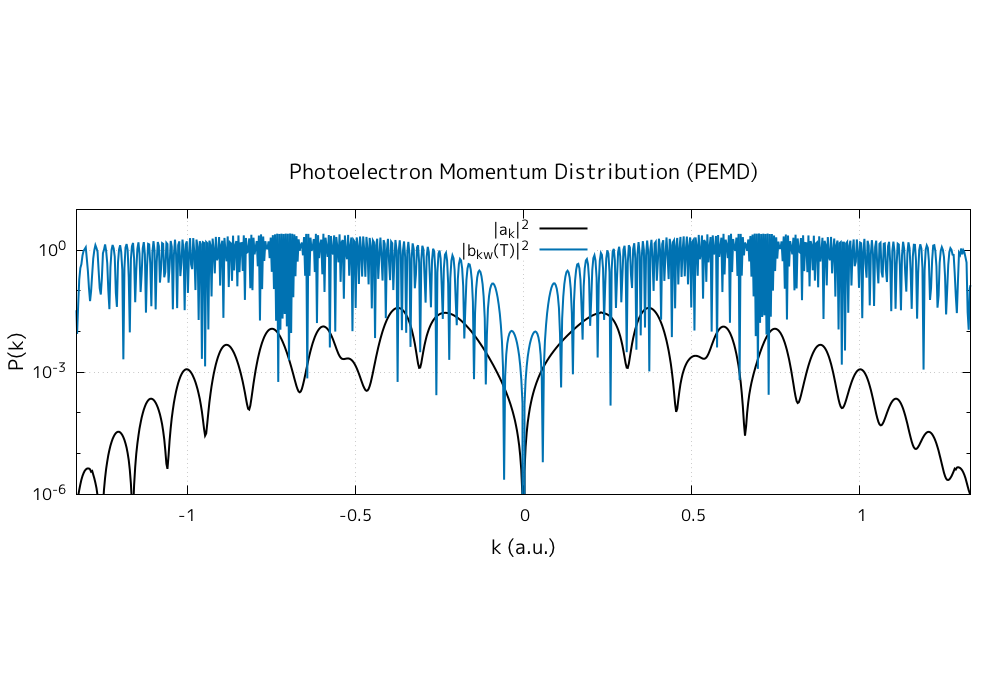
\includegraphics[scale=.18, trim={6 180 10 185},clip]{images/pemd_20_200_1000_2.png} \\
 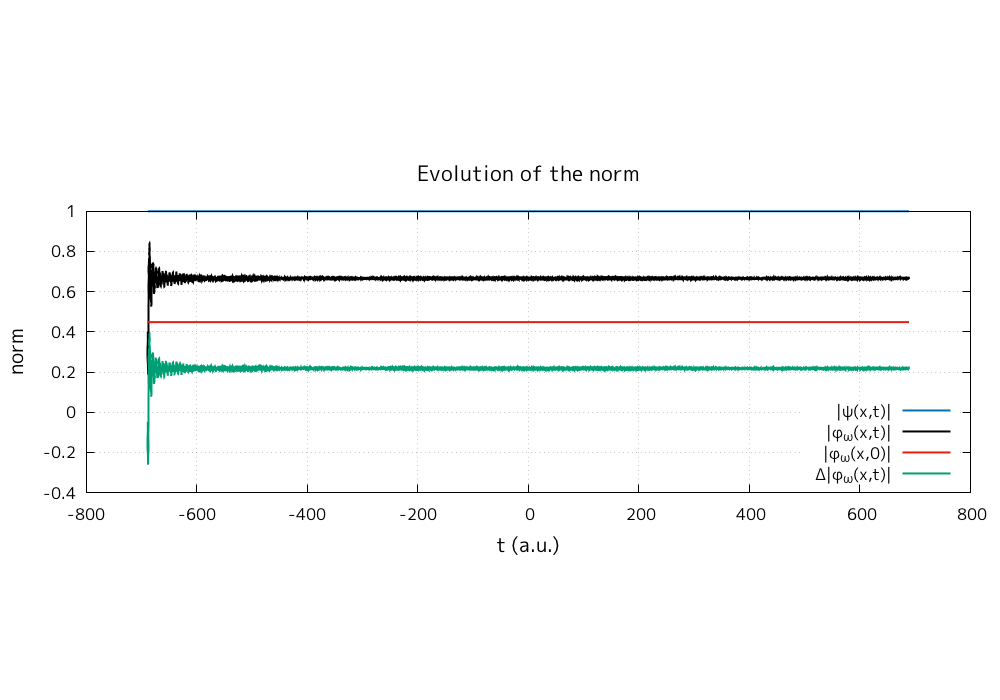
\includegraphics[scale=.18, trim={6 150 10 185},clip]{images/norm_20_200_20k_1q10.png} \\
% \includegraphics[scale=.18, trim={6 140 10 185},clip]{/s/fred/ドキュメント/電通大/hpc_fedvr_main_ref/data/exp/png_density/density_003_114_20k_25_30_200_2.png} 
%%\caption{Eigenvalues.}
%\label{fig:pemd_0114}
 \end{figure}

\end{minipage}
\end{textblock*}


\begin{textblock*}{500pt}(190pt,60pt)
%\centering
%\rotatebox{90}{
 \begin{minipage}{0.0\linewidth}
% \begin{figure}[tp]
% 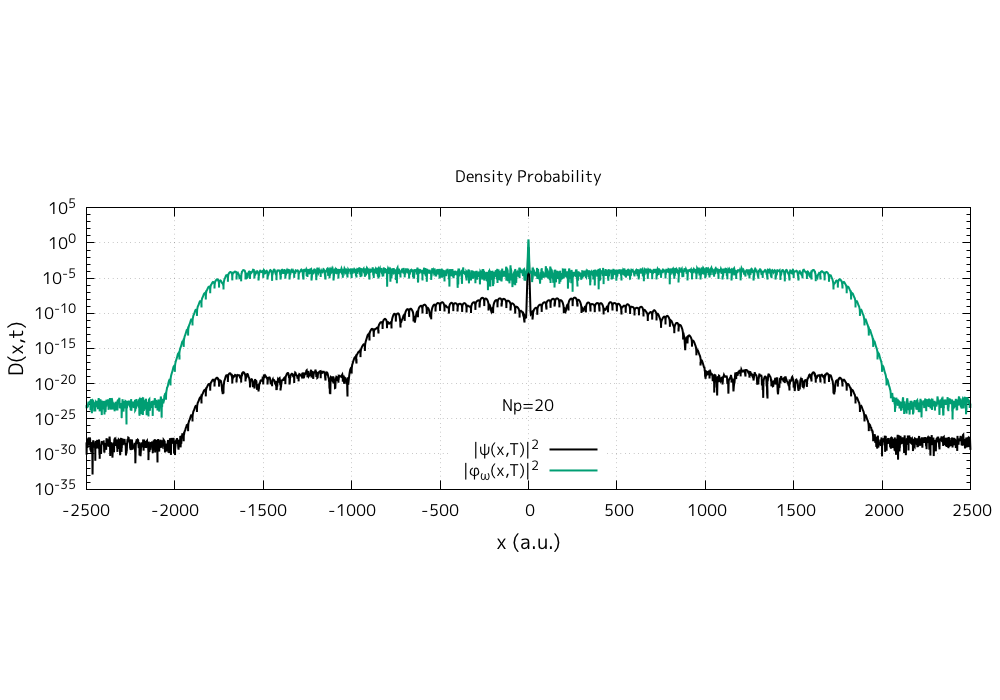
\includegraphics[scale=.18, trim={6 180 10 185},clip]{images/density_comp_file_1q4_np20.png} \\
% 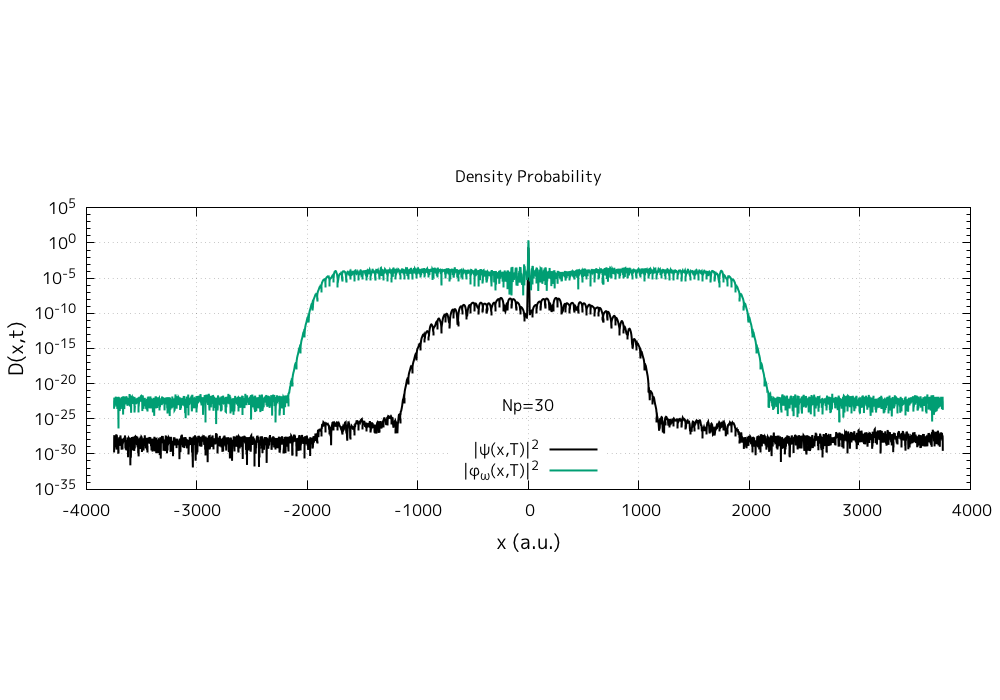
\includegraphics[scale=.18, trim={6 150 10 185},clip]{images/density_comp_file_1q4_np30.png} \\
%% 
\includegraphics[scale=.20, trim={30 130 10 130},clip]{images/114_f003_12_07_hhg.png} 
%%%\caption{Eigenvalues.}
%%\label{fig:pemd_0114}
% \end{figure}

\end{minipage}
\end{textblock*}


%

\begin{textblock*}{200pt}(260pt,130pt)
\rotatebox{0}{
\begin{minipage}{\linewidth}
{
\scriptsize
\centering


\footnotesize
\begin{align}
  Q(\omega) = \left| b_{0\omega}\right|^2
        + \int \left| b_{k\omega}\right|^2 \frac{dk}{2\pi} \nonumber
\end{align}
        \begin{align}
                \rm{Np} = 20,\;\;\;\rm{Ns} = 200 \nonumber\\
%               \;\;\;\rm{Ns} = 200 \nonumber\\
                \rm{xmax} \sim \left(\rm{Np\,Ns}+q\right)/2 \nonumber\\
                \omega_0 = 0.114\,{\rm a.u}\nonumber\\
                q=1/10\nonumber\\
                F_0 = 0.03\,{\rm a.u}, \;\;T=5\tau\nonumber\\
                {\rm nsteps} = 20 000,\, \;\;\Delta t=0.06889\nonumber
        \end{align}
%       \textcolor{red}{\textbf{The nonconvergence come from the fact that}
%       $\rm{xmax}\sim \rm{Np\,Ns}$ here}

}
\end{minipage}
}
\end{textblock*}



\begin{textblock*}{200pt}(270pt,80pt)
\rotatebox{0}{
\begin{minipage}{\linewidth}
{
\scriptsize
\centering

\footnotesize
\begin{align}
b_{0\omega}(T) & = e^{iE_0T} \int \psi_0(x) \phi_\omega(x,T) dx, \nonumber \\
b_{k\omega}(T) & = e^{iE_kT} \int \psi_k^{(-)*}(x) \phi_\omega(x,T) dx\nonumber,
\end{align}
}
\end{minipage}
}
\end{textblock*}



\begin{textblock*}{200pt}(30pt,190pt)
\footnotesize

\begin{align}
b_{0\omega} & = b_{0\omega}(T)
 +\int\frac{e^{i(E_0+\omega-E_{k^\prime})T}p_{0k^\prime}a_{k^\prime}}
{E_0+\omega-E_{k^\prime} + i0} \frac{dk^\prime}{2\pi} \nonumber\\
b_{k\omega} & = b_{k\omega}(T)
 +\frac{e^{i(E_k+\omega-E_0)T}p_{k0}a_0}{E_k+\omega-E_0}
 +\int\frac{e^{i(E_k+\omega-E_{k^\prime})T}p_{kk^\prime}a_{k^\prime}}
{E_k+\omega-E_{k^\prime} + i0} \frac{dk^\prime}{2\pi} \nonumber
\end{align}

%\begin{align}
% i\partial_t \phi_{\omega}(t) 
% & = \left(\hat{H}_a + \hat{V}_{\rm ext}(t) \right) \phi_{\omega}(t) \nonumber\\
% i\partial_t \phi_{\omega}(t) 
% & = \left(\hat{H}_a + \hat{V}_{\rm ext}(t) \right) \phi_{\omega}(t) 
%-i e^{i\omega t} \partial_x \psi (x,t) \nonumber
%\end{align}
%%\begin{itemize}
%\scriptsize
%\item The convergence region for $\psi$ is ${\rm xrange} \sim 2000$
%\item The convergence region for $\phi$ is ${\rm xrange} \sim 4500$
%\item The plateau for $\phi$ seems to be $1e-8$, 
%above the double precision limit
%\item The result is confirmed by 2 different methods and has been tested 
%against an analytical result
%\end{itemize}

\end{textblock*}


\end{frame}










\begin{frame}
\frametitle{Quantum theory of radiation by nonstationary systems 
        with application to high-order harmonic generation
        (Phys. Rev. A 101, 013410 (2020))}
        \framesubtitle{Quantum High Harmonic Generation, 
        for $\phi_\omega$ (many channels)... - Propagation program}
\small
\begin{textblock*}{500pt}(5pt,60pt)
%\centering
%\rotatebox{90}{
 \begin{minipage}{0.0\linewidth}
 \begin{figure}[tp]
% \includegraphics[scale=.18, trim={6 140 10 185},clip]{/s/fred/ドキュメント/電通大/hpc_fedvr_main_ref/data/exp/png_hhg/hhg_003_114_20k_25_30_200.png} \\
%% \includegraphics[scale=.18, trim={6 180 10 185},clip]{/s/fred/ドキュメント/電通大/hpc_fedvr_main_ref/data/exp/png_density/density_003_114_15k_25_30_200_2.png} \\
% \includegraphics[scale=.18, trim={6 140 10 185},clip]{/s/fred/ドキュメント/電通大/hpc_fedvr_main_ref/data/exp/png_hhg/bkw_003_114_20k_25_30_200.png} 
%%%\caption{Eigenvalues.}
%\label{fig:pemd_0114}
 \end{figure}

\end{minipage}
\end{textblock*}

%\begin{textblock*}{300pt}(100pt,180pt)
%\rotatebox{0}{
%\begin{minipage}{\linewidth}
%{
%\scriptsize
%For this laser intensity and frequency, the reference result is
%$Q(\omega) \sim 1e-5$ 
%}
%\end{minipage}
%}
%\end{textblock*}


\begin{textblock*}{\linewidth}(20pt,100pt)
\rotatebox{0}{
\begin{minipage}{\linewidth}
{
\Tiny
\input{tables/norm_multichan.tab}
}
\end{minipage}
}
\end{textblock*}

\begin{textblock*}{300pt}(100pt,160pt)
\rotatebox{0}{
\begin{minipage}{\linewidth}
{
\scriptsize
Solving the inhomogeneous equation for hundreds of channels simultaneously
}
\end{minipage}
}
\end{textblock*}

%
%
%\begin{textblock*}{200pt}(150pt,205pt)
%\scriptsize
%%
%\begin{align}
%	&Q^{(c)}(\omega) = \omega^2 \left| d(\omega)  \right|^2, \nonumber\\
%	&\mbox{Above is Eq.80, below is Eq.(104)} \nonumber\\
%        &Q^{(c)}(\omega) = \left| p(\omega)  \right|^2. \nonumber
%\end{align}
%
%
%\end{textblock*}

\end{frame}






\begin{frame}
\frametitle{Quantum theory of radiation by nonstationary systems 
        with application to high-order harmonic generation
        (Phys. Rev. A 101, 013410 (2020))}
        \framesubtitle{Quantum High Harmonic Generation, 
        for $\phi_\omega$ (many channels)... - Exploitation program}
\small
\begin{textblock*}{500pt}(5pt,60pt)
%\centering
%\rotatebox{90}{
 \begin{minipage}{0.0\linewidth}
 \begin{figure}[tp]
% \includegraphics[scale=.18, trim={6 140 10 185},clip]{/s/fred/ドキュメント/電通大/hpc_fedvr_main_ref/data/exp/png_hhg/hhg_003_114_20k_25_30_200.png} \\
%% \includegraphics[scale=.18, trim={6 180 10 185},clip]{/s/fred/ドキュメント/電通大/hpc_fedvr_main_ref/data/exp/png_density/density_003_114_15k_25_30_200_2.png} \\
% \includegraphics[scale=.18, trim={6 140 10 185},clip]{/s/fred/ドキュメント/電通大/hpc_fedvr_main_ref/data/exp/png_hhg/bkw_003_114_20k_25_30_200.png} 
%%%\caption{Eigenvalues.}
%\label{fig:pemd_0114}
 \end{figure}

\end{minipage}
\end{textblock*}

\begin{textblock*}{300pt}(100pt,137pt)
\rotatebox{0}{
\begin{minipage}{\linewidth}
{
\scriptsize
For this laser intensity and frequency, the reference result is
$Q(\omega) \sim 1e-5$ 
}
\end{minipage}
}
\end{textblock*}


\begin{textblock*}{\linewidth}(20pt,100pt)
\rotatebox{0}{
\begin{minipage}{\linewidth}
{
\Tiny
\input{tables/Qw.tab}
\input{tables/Qw_.tab}
}
\end{minipage}
}
\end{textblock*}
%
%
%\begin{textblock*}{200pt}(150pt,205pt)
%\scriptsize
%%
%\begin{align}
%	&Q^{(c)}(\omega) = \omega^2 \left| d(\omega)  \right|^2, \nonumber\\
%	&\mbox{Above is Eq.80, below is Eq.(104)} \nonumber\\
%        &Q^{(c)}(\omega) = \left| p(\omega)  \right|^2. \nonumber
%\end{align}
%
%
%\end{textblock*}

\end{frame}





\begin{frame}
\frametitle{Quantum theory of radiation by nonstationary systems 
        with application to high-order harmonic generation
        (Phys. Rev. A 101, 013410 (2020))}
        \framesubtitle{Q-HHG vs C-HHG}
\small
\begin{textblock*}{500pt}(5pt,60pt)
%\centering
%\rotatebox{90}{
 \begin{minipage}{0.0\linewidth}
 \begin{figure}[tp]
 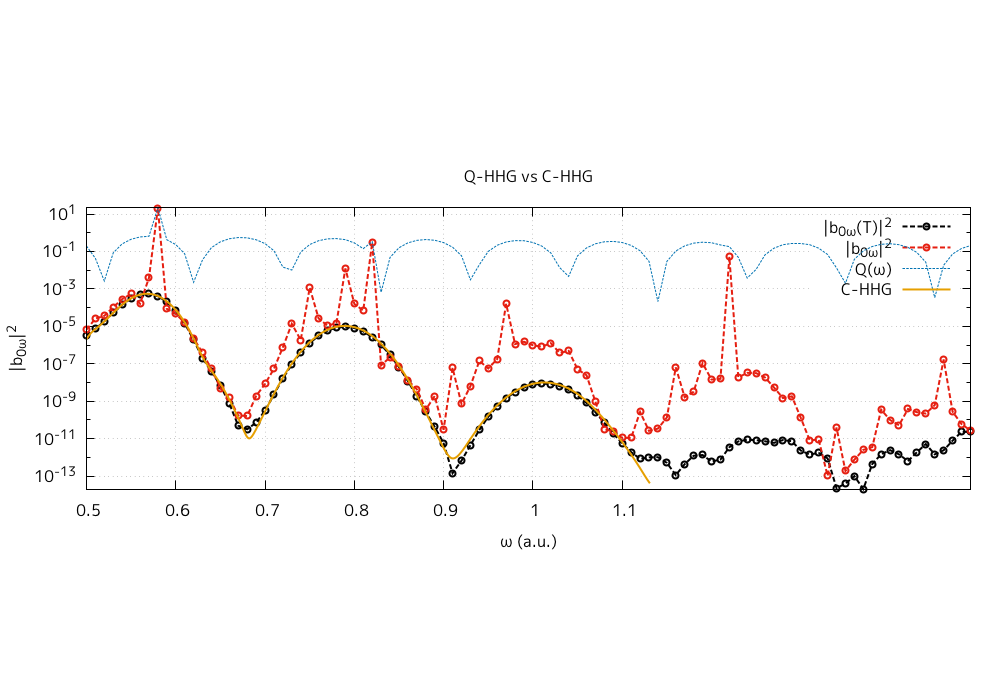
\includegraphics[scale=.28, trim={6 140 10 185},clip]{images/components_20_200_hhg_b0w.png} \\
%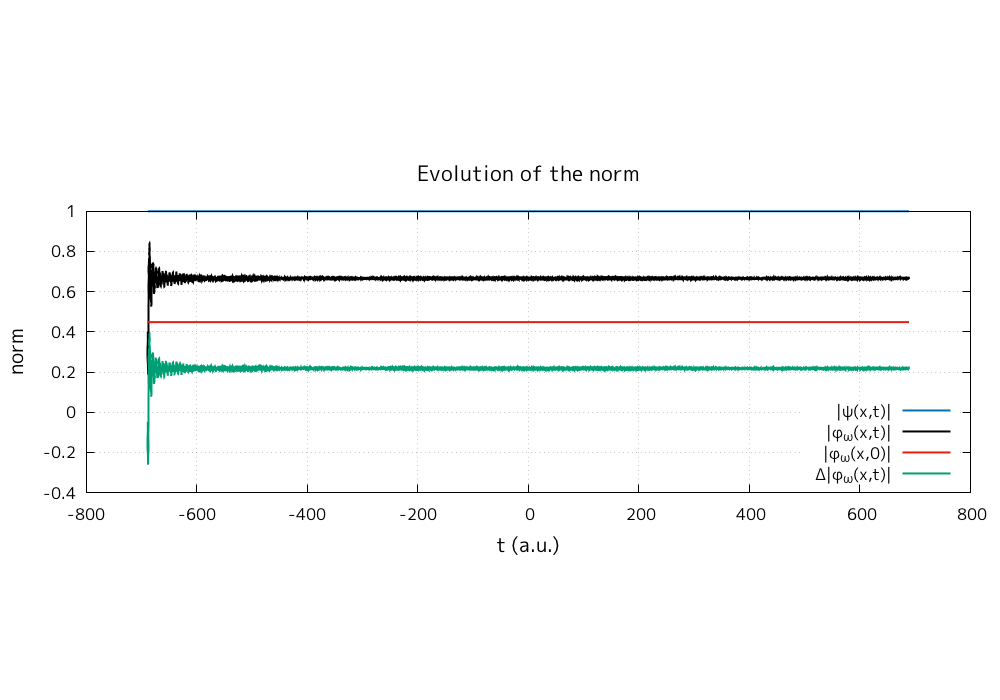
\includegraphics[scale=.18, trim={6 150 10 185},clip]{images/norm_20_200_20k_1q10.png} \\
% \includegraphics[scale=.18, trim={6 140 10 185},clip]{/s/fred/ドキュメント/電通大/hpc_fedvr_main_ref/data/exp/png_density/density_003_114_20k_25_30_200_2.png} 
%%\caption{Eigenvalues.}
%\label{fig:pemd_0114}
 \end{figure}

\end{minipage}
\end{textblock*}


\begin{textblock*}{500pt}(190pt,60pt)
%\centering
%\rotatebox{90}{
 \begin{minipage}{0.0\linewidth}
% \begin{figure}[tp]
% 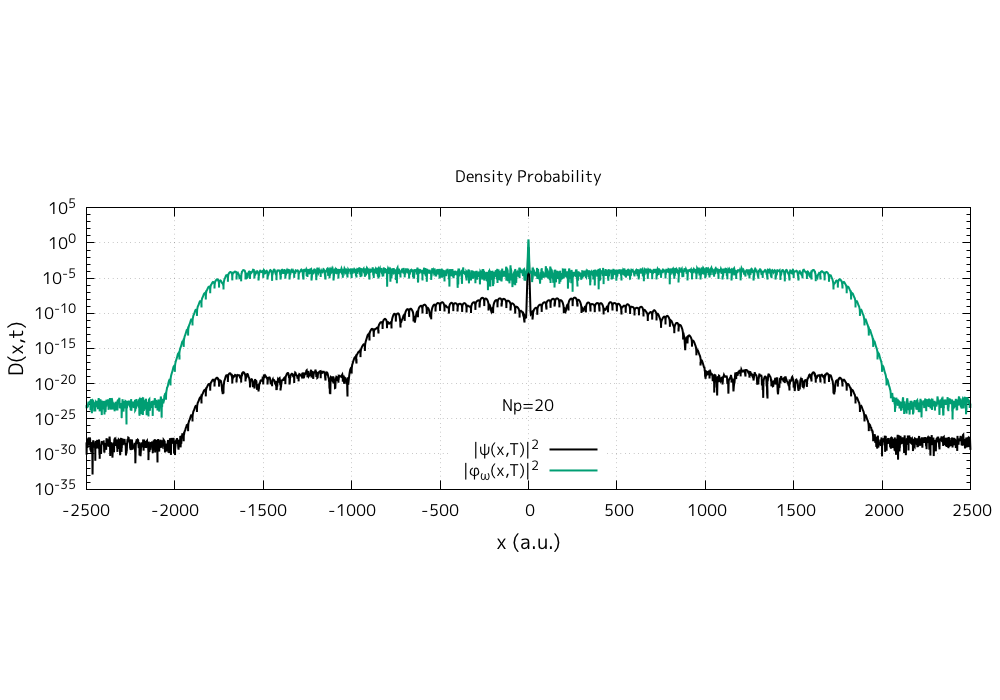
\includegraphics[scale=.18, trim={6 180 10 185},clip]{images/density_comp_file_1q4_np20.png} \\
% 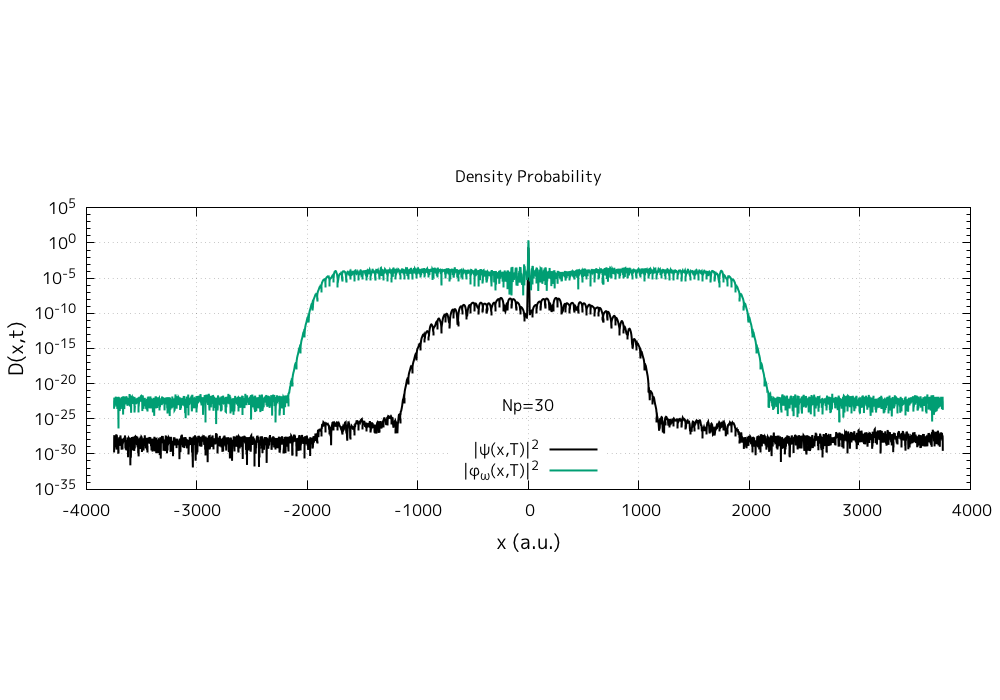
\includegraphics[scale=.18, trim={6 150 10 185},clip]{images/density_comp_file_1q4_np30.png} \\
%% 
\includegraphics[scale=.20, trim={30 130 10 130},clip]{images/114_f003_12_07_hhg.png} 
%%%\caption{Eigenvalues.}
%%\label{fig:pemd_0114}
% \end{figure}

\end{minipage}
\end{textblock*}


%
\begin{textblock*}{200pt}(270pt,80pt)
\rotatebox{0}{
\begin{minipage}{\linewidth}
{
\scriptsize
\centering

\footnotesize
\begin{align}
b_{0\omega}(T) & = e^{iE_0T} \int \psi_0(x) \phi_\omega(x,T) dx, \nonumber \\
b_{k\omega}(T) & = e^{iE_kT} \int \psi_k^{(-)*}(x) \phi_\omega(x,T) dx\nonumber,
\end{align}
}
\end{minipage}
}
\end{textblock*}


\begin{textblock*}{200pt}(260pt,130pt)
\rotatebox{0}{
\begin{minipage}{\linewidth}
{
\scriptsize
\centering


\footnotesize
\begin{align}
  Q(\omega) = \left| b_{0\omega}\right|^2
        + \int \left| b_{k\omega}\right|^2 \frac{dk}{2\pi} \nonumber
\end{align}
        \begin{align}
                \rm{Np} = 20,\;\;\;\rm{Ns} = 200 \nonumber\\
%               \;\;\;\rm{Ns} = 200 \nonumber\\
                \rm{xmax} \sim \left(\rm{Np\,Ns}+q\right)/2 \nonumber\\
                \omega_0 = 0.114\,{\rm a.u}\nonumber\\
                q=1/10\nonumber\\
                F_0 = 0.03\,{\rm a.u}, \;\;T=5\tau\nonumber\\
                {\rm nsteps} = 20 000,\, \;\;\Delta t=0.06889\nonumber
        \end{align}
%       \textcolor{red}{\textbf{The nonconvergence come from the fact that}
%       $\rm{xmax}\sim \rm{Np\,Ns}$ here}

}
\end{minipage}
}
\end{textblock*}


\begin{textblock*}{200pt}(30pt,190pt)
\footnotesize

\begin{align}
b_{0\omega} & = b_{0\omega}(T)
 +\int\frac{e^{i(E_0+\omega-E_{k^\prime})T}p_{0k^\prime}a_{k^\prime}}
{E_0+\omega-E_{k^\prime} + i0} \frac{dk^\prime}{2\pi} \nonumber\\
b_{k\omega} & = b_{k\omega}(T)
 +\frac{e^{i(E_k+\omega-E_0)T}p_{k0}a_0}{E_k+\omega-E_0}
 +\int\frac{e^{i(E_k+\omega-E_{k^\prime})T}p_{kk^\prime}a_{k^\prime}}
{E_k+\omega-E_{k^\prime} + i0} \frac{dk^\prime}{2\pi} \nonumber
\end{align}

%\begin{align}
% i\partial_t \phi_{\omega}(t) 
% & = \left(\hat{H}_a + \hat{V}_{\rm ext}(t) \right) \phi_{\omega}(t) \nonumber\\
% i\partial_t \phi_{\omega}(t) 
% & = \left(\hat{H}_a + \hat{V}_{\rm ext}(t) \right) \phi_{\omega}(t) 
%-i e^{i\omega t} \partial_x \psi (x,t) \nonumber
%\end{align}
%%\begin{itemize}
%\scriptsize
%\item The convergence region for $\psi$ is ${\rm xrange} \sim 2000$
%\item The convergence region for $\phi$ is ${\rm xrange} \sim 4500$
%\item The plateau for $\phi$ seems to be $1e-8$, 
%above the double precision limit
%\item The result is confirmed by 2 different methods and has been tested 
%against an analytical result
%\end{itemize}

\end{textblock*}


\end{frame}










\begin{frame}
\frametitle{Quantum theory of radiation by nonstationary systems 
        with application to high-order harmonic generation
        (Phys. Rev. A 101, 013410 (2020))}
        \framesubtitle{Study of the the coefficients 
        $b_{k\omega}(T)$ and $b_{k\omega}$}
\small
\begin{textblock*}{500pt}(5pt,60pt)
%\centering
%\rotatebox{90}{
 \begin{minipage}{0.0\linewidth}
 \begin{figure}[tp]
 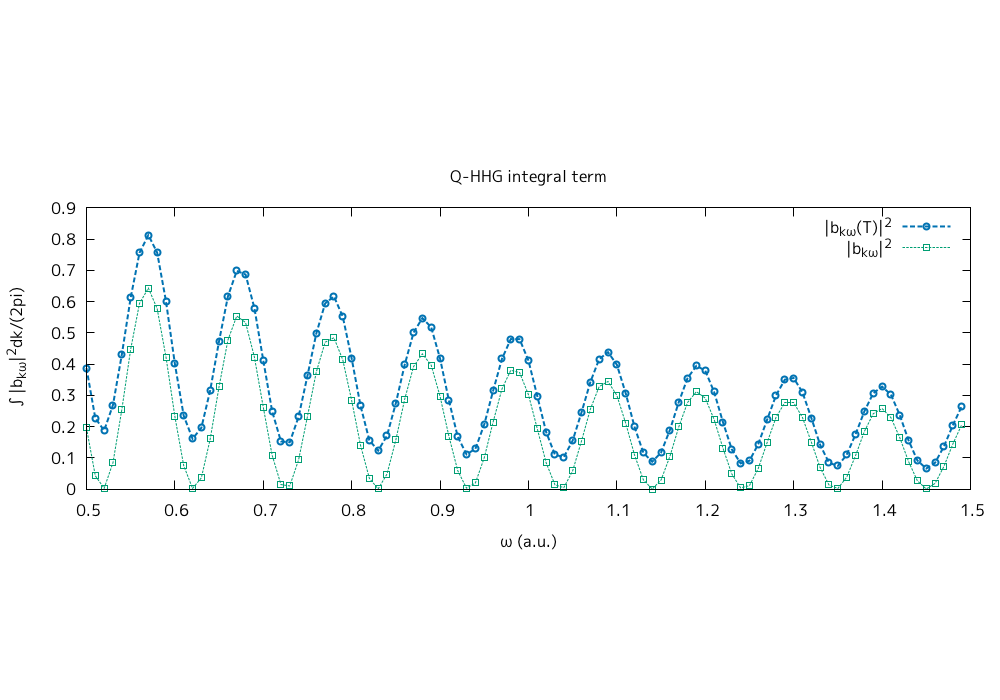
\includegraphics[scale=.18, trim={6 180 10 185},clip]{images/components_20_200_hhg_bkw.png} \\
 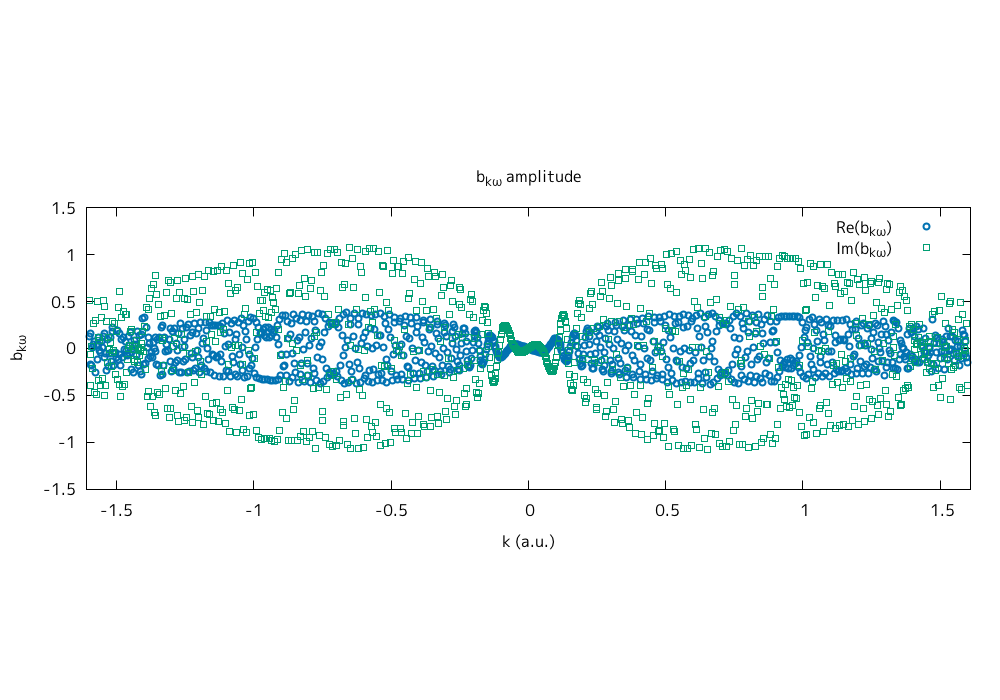
\includegraphics[scale=.18, trim={6 150 10 185},clip]{images/components_20_200_bkw_bkwT.png} \\
% \includegraphics[scale=.18, trim={6 140 10 185},clip]{/s/fred/ドキュメント/電通大/hpc_fedvr_main_ref/data/exp/png_density/density_003_114_20k_25_30_200_2.png} 
%%\caption{Eigenvalues.}
%\label{fig:pemd_0114}
 \end{figure}

\end{minipage}
\end{textblock*}


\begin{textblock*}{500pt}(190pt,60pt)
%\centering
%\rotatebox{90}{
 \begin{minipage}{0.0\linewidth}
% \begin{figure}[tp]
% 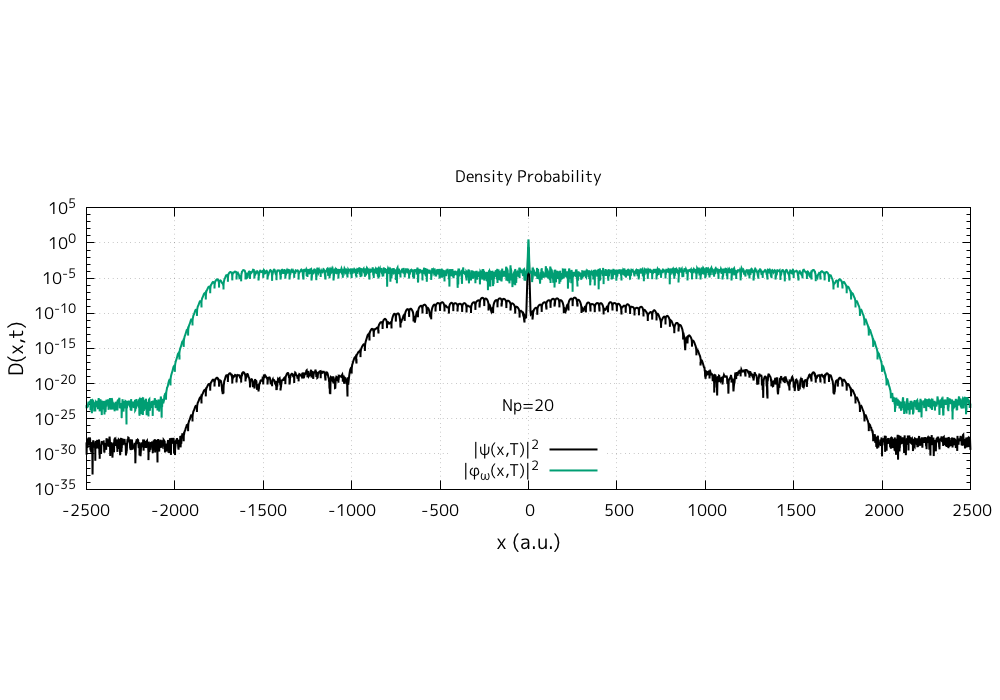
\includegraphics[scale=.18, trim={6 180 10 185},clip]{images/density_comp_file_1q4_np20.png} \\
% 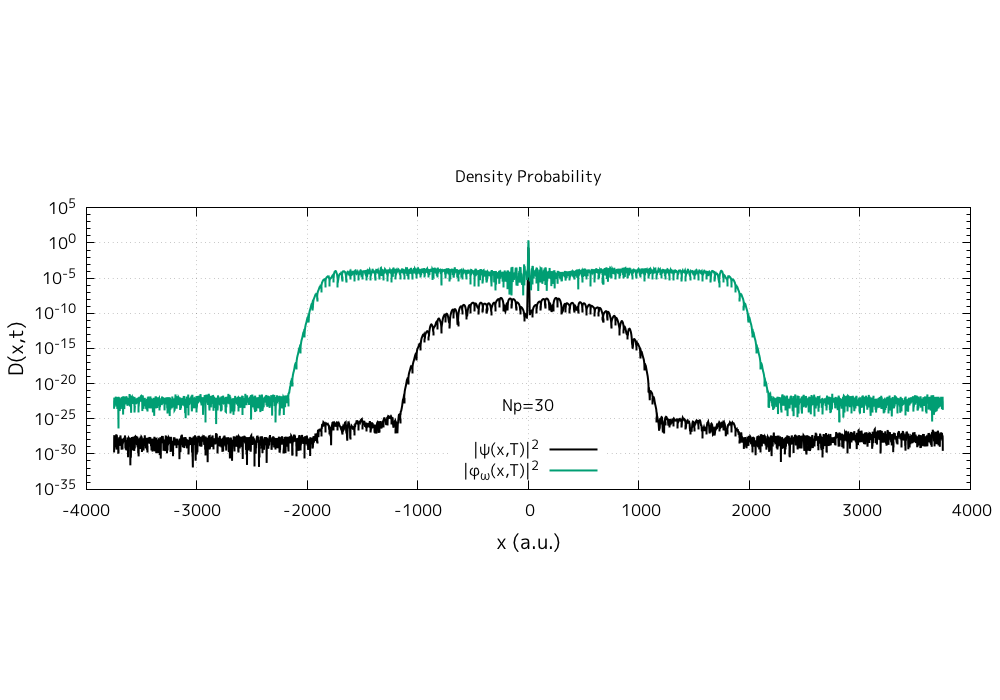
\includegraphics[scale=.18, trim={6 150 10 185},clip]{images/density_comp_file_1q4_np30.png} \\
%% 
\includegraphics[scale=.20, trim={30 130 10 130},clip]{images/114_f003_12_07_hhg.png} 
%%%\caption{Eigenvalues.}
%%\label{fig:pemd_0114}
% \end{figure}

\end{minipage}
\end{textblock*}


\begin{textblock*}{200pt}(270pt,80pt)
\rotatebox{0}{
\begin{minipage}{\linewidth}
{
\scriptsize
\centering

\footnotesize
\begin{align}
b_{0\omega}(T) & = e^{iE_0T} \int \psi_0(x) \phi_\omega(x,T) dx, \nonumber \\
b_{k\omega}(T) & = e^{iE_kT} \int \psi_k^{(-)*}(x) \phi_\omega(x,T) dx\nonumber,
\end{align}
}
\end{minipage}
}
\end{textblock*}



\begin{textblock*}{200pt}(260pt,130pt)
\rotatebox{0}{
\begin{minipage}{\linewidth}
{
\scriptsize
\centering


\footnotesize
\begin{align}
  Q(\omega) = \left| b_{0\omega}\right|^2
        + \int \left| b_{k\omega}\right|^2 \frac{dk}{2\pi} \nonumber
\end{align}
        \begin{align}
                \rm{Np} = 20,\;\;\;\rm{Ns} = 200 \nonumber\\
%               \;\;\;\rm{Ns} = 200 \nonumber\\
                \rm{xmax} \sim \left(\rm{Np\,Ns}+q\right)/2 \nonumber\\
                \omega_0 = 0.114\,{\rm a.u}\nonumber\\
                q=1/10\nonumber\\
                F_0 = 0.03\,{\rm a.u}, \;\;T=5\tau\nonumber\\
                {\rm nsteps} = 20 000,\, \;\;\Delta t=0.06889\nonumber
        \end{align}
%       \textcolor{red}{\textbf{The nonconvergence come from the fact that}
%       $\rm{xmax}\sim \rm{Np\,Ns}$ here}

}
\end{minipage}
}
\end{textblock*}





\begin{textblock*}{200pt}(30pt,190pt)
\footnotesize

\begin{align}
b_{0\omega} & = b_{0\omega}(T)
 +\int\frac{e^{i(E_0+\omega-E_{k^\prime})T}p_{0k^\prime}a_{k^\prime}}
{E_0+\omega-E_{k^\prime} + i0} \frac{dk^\prime}{2\pi} \nonumber\\
b_{k\omega} & = b_{k\omega}(T)
 +\frac{e^{i(E_k+\omega-E_0)T}p_{k0}a_0}{E_k+\omega-E_0}
 +\int\frac{e^{i(E_k+\omega-E_{k^\prime})T}p_{kk^\prime}a_{k^\prime}}
{E_k+\omega-E_{k^\prime} + i0} \frac{dk^\prime}{2\pi} \nonumber
\end{align}

%\begin{align}
% i\partial_t \phi_{\omega}(t) 
% & = \left(\hat{H}_a + \hat{V}_{\rm ext}(t) \right) \phi_{\omega}(t) \nonumber\\
% i\partial_t \phi_{\omega}(t) 
% & = \left(\hat{H}_a + \hat{V}_{\rm ext}(t) \right) \phi_{\omega}(t) 
%-i e^{i\omega t} \partial_x \psi (x,t) \nonumber
%\end{align}
%%\begin{itemize}
%\scriptsize
%\item The convergence region for $\psi$ is ${\rm xrange} \sim 2000$
%\item The convergence region for $\phi$ is ${\rm xrange} \sim 4500$
%\item The plateau for $\phi$ seems to be $1e-8$, 
%above the double precision limit
%\item The result is confirmed by 2 different methods and has been tested 
%against an analytical result
%\end{itemize}

\end{textblock*}


\end{frame}





\begin{frame}
\frametitle{Quantum theory of radiation by nonstationary systems 
        with application to high-order harmonic generation
        (Phys. Rev. A 101, 013410 (2020))}
        \framesubtitle{Study of the 
        structure dependent integral terms (futatabi)}
\small
\begin{textblock*}{500pt}(5pt,60pt)
%\centering
%\rotatebox{90}{
 \begin{minipage}{0.0\linewidth}
 \begin{figure}[tp]
 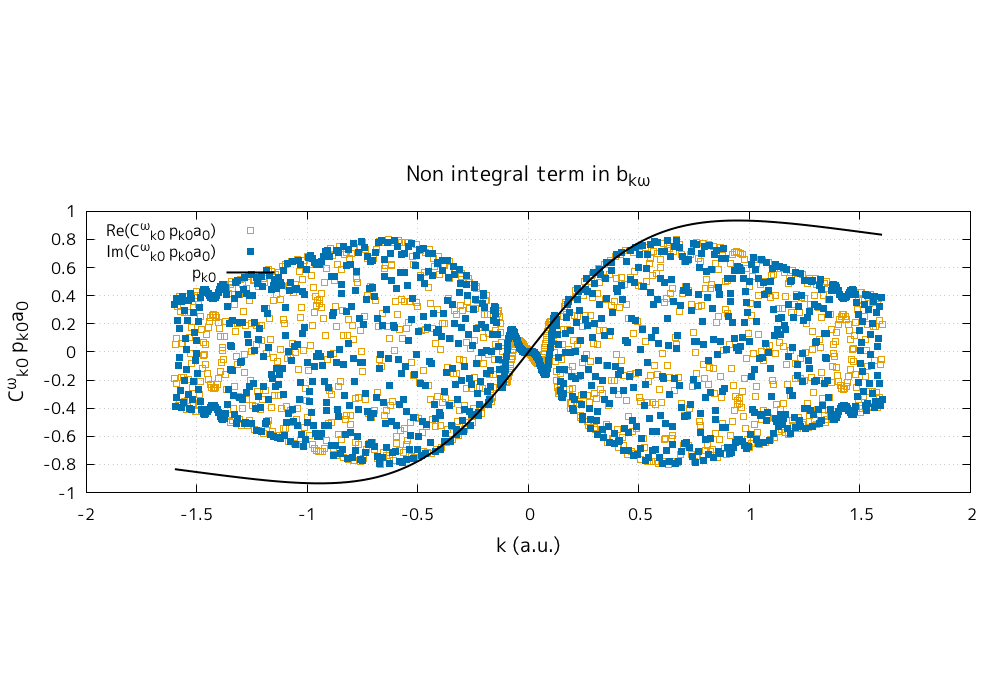
\includegraphics[scale=.18, trim={6 180 10 185},clip]{images/diff_terms_pk0a0.png} \\
 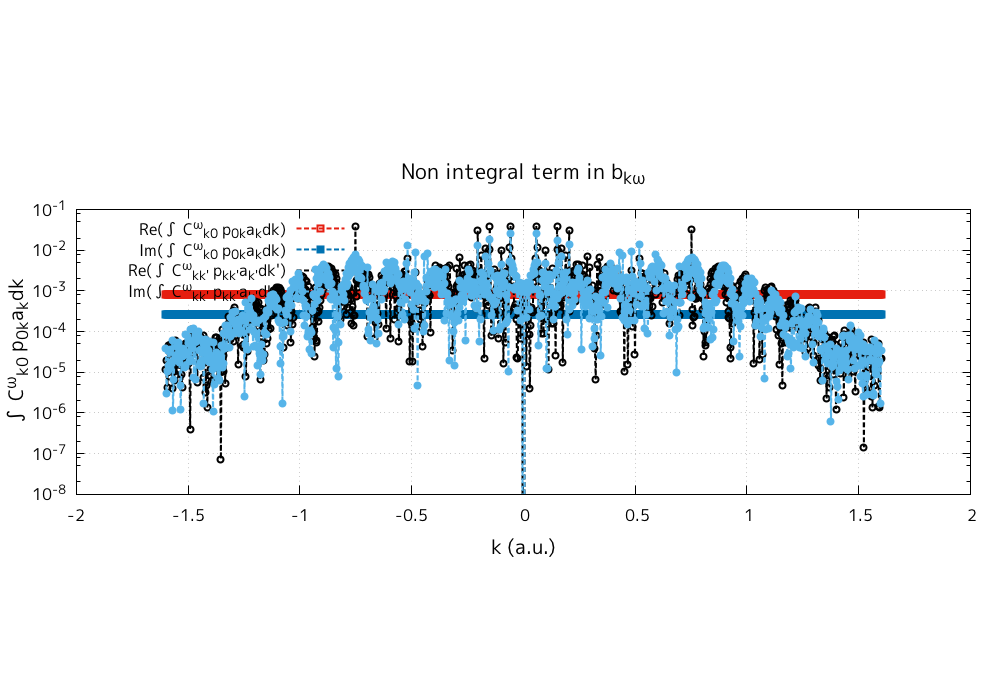
\includegraphics[scale=.18, trim={6 150 10 185},clip]{images/diff_terms_pkkak_1.png} \\
% \includegraphics[scale=.18, trim={6 140 10 185},clip]{/s/fred/ドキュメント/電通大/hpc_fedvr_main_ref/data/exp/png_density/density_003_114_20k_25_30_200_2.png} 
%%\caption{Eigenvalues.}
%\label{fig:pemd_0114}
 \end{figure}

\end{minipage}
\end{textblock*}


\begin{textblock*}{500pt}(190pt,60pt)
%\centering
%\rotatebox{90}{
 \begin{minipage}{0.0\linewidth}
% \begin{figure}[tp]
% 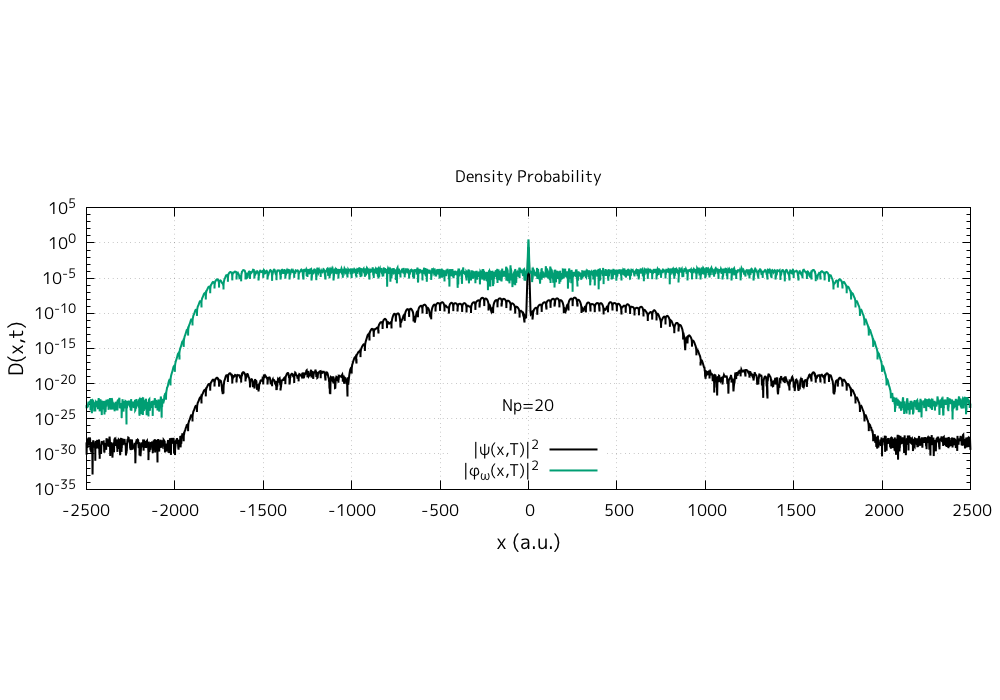
\includegraphics[scale=.18, trim={6 180 10 185},clip]{images/density_comp_file_1q4_np20.png} \\
% 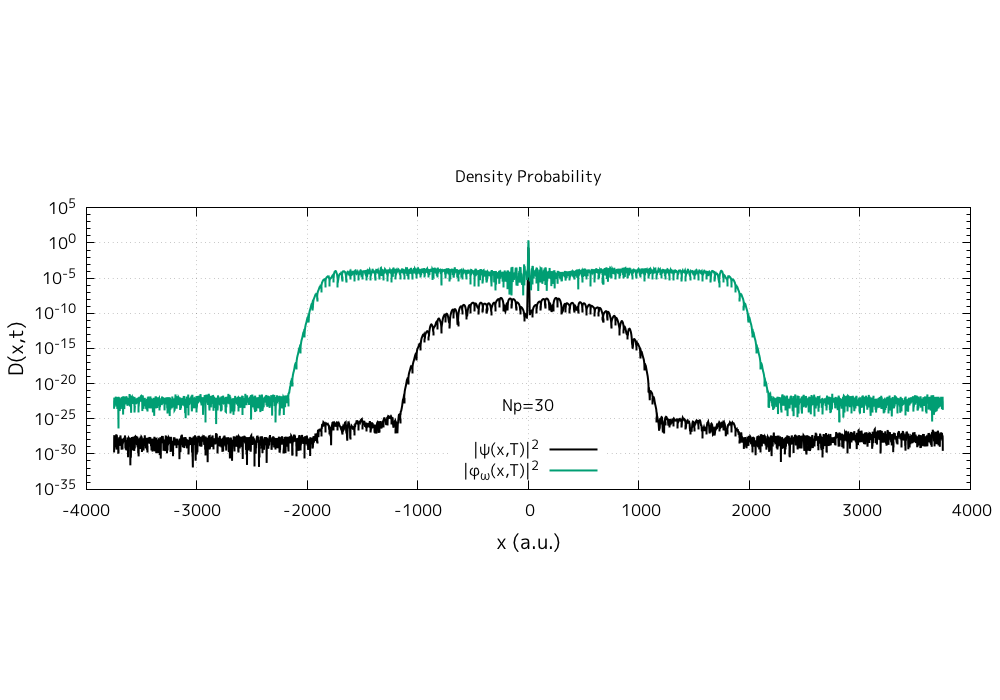
\includegraphics[scale=.18, trim={6 150 10 185},clip]{images/density_comp_file_1q4_np30.png} \\
%% 
\includegraphics[scale=.20, trim={30 130 10 130},clip]{images/114_f003_12_07_hhg.png} 
%%%\caption{Eigenvalues.}
%%\label{fig:pemd_0114}
% \end{figure}

\end{minipage}
\end{textblock*}


\begin{textblock*}{200pt}(270pt,80pt)
\rotatebox{0}{
\begin{minipage}{\linewidth}
{
\scriptsize
\centering

\footnotesize
\begin{align}
b_{0\omega}(T) & = e^{iE_0T} \int \psi_0(x) \phi_\omega(x,T) dx, \nonumber \\
b_{k\omega}(T) & = e^{iE_kT} \int \psi_k^{(-)*}(x) \phi_\omega(x,T) dx\nonumber,
\end{align}
}
\end{minipage}
}
\end{textblock*}



\begin{textblock*}{200pt}(260pt,130pt)
\rotatebox{0}{
\begin{minipage}{\linewidth}
{
\scriptsize
\centering


\footnotesize
\begin{align}
  Q(\omega) = \left| b_{0\omega}\right|^2
        + \int \left| b_{k\omega}\right|^2 \frac{dk}{2\pi} \nonumber
\end{align}
        \begin{align}
                \rm{Np} = 20,\;\;\;\rm{Ns} = 200 \nonumber\\
%               \;\;\;\rm{Ns} = 200 \nonumber\\
                \rm{xmax} \sim \left(\rm{Np\,Ns}+q\right)/2 \nonumber\\
                \omega_0 = 0.114\,{\rm a.u}\nonumber\\
                q=1/10\nonumber\\
                F_0 = 0.03\,{\rm a.u}, \;\;T=5\tau\nonumber\\
                {\rm nsteps} = 20 000,\, \;\;\Delta t=0.06889\nonumber
        \end{align}
%       \textcolor{red}{\textbf{The nonconvergence come from the fact that}
%       $\rm{xmax}\sim \rm{Np\,Ns}$ here}

}
\end{minipage}
}
\end{textblock*}





\begin{textblock*}{200pt}(30pt,190pt)
\footnotesize

\begin{align}
b_{0\omega} & = b_{0\omega}(T)
 +\int\frac{e^{i(E_0+\omega-E_{k^\prime})T}p_{0k^\prime}a_{k^\prime}}
{E_0+\omega-E_{k^\prime} + i0} \frac{dk^\prime}{2\pi} \nonumber\\
b_{k\omega} & = b_{k\omega}(T)
 +\frac{e^{i(E_k+\omega-E_0)T}p_{k0}a_0}{E_k+\omega-E_0}
 +\int\frac{e^{i(E_k+\omega-E_{k^\prime})T}p_{kk^\prime}a_{k^\prime}}
{E_k+\omega-E_{k^\prime} + i0} \frac{dk^\prime}{2\pi} \nonumber
\end{align}

%\begin{align}
% i\partial_t \phi_{\omega}(t) 
% & = \left(\hat{H}_a + \hat{V}_{\rm ext}(t) \right) \phi_{\omega}(t) \nonumber\\
% i\partial_t \phi_{\omega}(t) 
% & = \left(\hat{H}_a + \hat{V}_{\rm ext}(t) \right) \phi_{\omega}(t) 
%-i e^{i\omega t} \partial_x \psi (x,t) \nonumber
%\end{align}
%%\begin{itemize}
%\scriptsize
%\item The convergence region for $\psi$ is ${\rm xrange} \sim 2000$
%\item The convergence region for $\phi$ is ${\rm xrange} \sim 4500$
%\item The plateau for $\phi$ seems to be $1e-8$, 
%above the double precision limit
%\item The result is confirmed by 2 different methods and has been tested 
%against an analytical result
%\end{itemize}

\end{textblock*}


\end{frame}




\begin{frame}
\frametitle{Quantum theory of radiation by nonstationary systems 
        with application to high-order harmonic generation
        (Phys. Rev. A 101, 013410 (2020))}
        \framesubtitle{Coefficient $b_{0\omega}$ and $b_{k\omega}$ convergence}

\begin{textblock*}{400pt}(30pt,60pt)
\small

\begin{itemize}
\footnotesize
\item The value of $Q(\omega)$ for $\omega=0.5\,\rm a.u$
is taken as a reference
\begin{itemize}
\footnotesize
\item[$\bullet$] The converged value is of the order of $\sim 1e-5$
\item[$\bullet$] $Q(\omega)$ is the sum of two terms, the biggest 
has to be of the above order as a criterion 
\item[$\bullet$] $\int |b_{k{\omega}}|^2dk/(2\pi)$ outweight the required 
order. It indicates the direction to look for
\item[$\bullet$] $|b_{0{\omega}}|^2$ is likely correct ;
which suggests the wavefunction $\phi_\omega$ is  
\end{itemize}
\item This now looks like a convergence problem
\begin{itemize}
\footnotesize
\item[$\bullet$] likely in $k$
\item[$\bullet$] a faster converging gauge 
or the analytic expression will be tested for the transition terms 
\end{itemize}
\end{itemize}
\end{textblock*}



\begin{textblock*}{200pt}(30pt,190pt)
\footnotesize

\begin{align}
b_{0\omega} & = b_{0\omega}(T)
 +\int\frac{e^{i(E_0+\omega-E_{k^\prime})T}p_{0k^\prime}a_{k^\prime}}
{E_0+\omega-E_{k^\prime} + i0} \frac{dk^\prime}{2\pi} \nonumber\\
b_{k\omega} & = b_{k\omega}(T)
 +\frac{e^{i(E_k+\omega-E_0)T}p_{k0}a_0}{E_k+\omega-E_0}
 +\int\frac{e^{i(E_k+\omega-E_{k^\prime})T}p_{kk^\prime}a_{k^\prime}}
{E_k+\omega-E_{k^\prime} + i0} \frac{dk^\prime}{2\pi} \nonumber
\end{align}

%\begin{align}
% i\partial_t \phi_{\omega}(t) 
% & = \left(\hat{H}_a + \hat{V}_{\rm ext}(t) \right) \phi_{\omega}(t) \nonumber\\
% i\partial_t \phi_{\omega}(t) 
% & = \left(\hat{H}_a + \hat{V}_{\rm ext}(t) \right) \phi_{\omega}(t) 
%-i e^{i\omega t} \partial_x \psi (x,t) \nonumber
%\end{align}
%%\begin{itemize}
%\scriptsize
%\item The convergence region for $\psi$ is ${\rm xrange} \sim 2000$
%\item The convergence region for $\phi$ is ${\rm xrange} \sim 4500$
%\item The plateau for $\phi$ seems to be $1e-8$, 
%above the double precision limit
%\item The result is confirmed by 2 different methods and has been tested 
%against an analytical result
%\end{itemize}

\end{textblock*}



\end{frame}











%\begin{frame}
%
%\frametitle{Quantum theory of radiation by nonstationary systems 
%	with application to high-order harmonic generation
%        (Phys. Rev. A 101, 013410 (2020))}
%	\framesubtitle{Self conv. test results for real tests, both orders}
%
%\footnotesize
%
%
%\begin{textblock*}{\linewidth}(0pt,60pt)
%\rotatebox{0}{
%\begin{minipage}{.5\linewidth}
%\Tiny
%\raggedright
% \begin{figure}[tp]
% 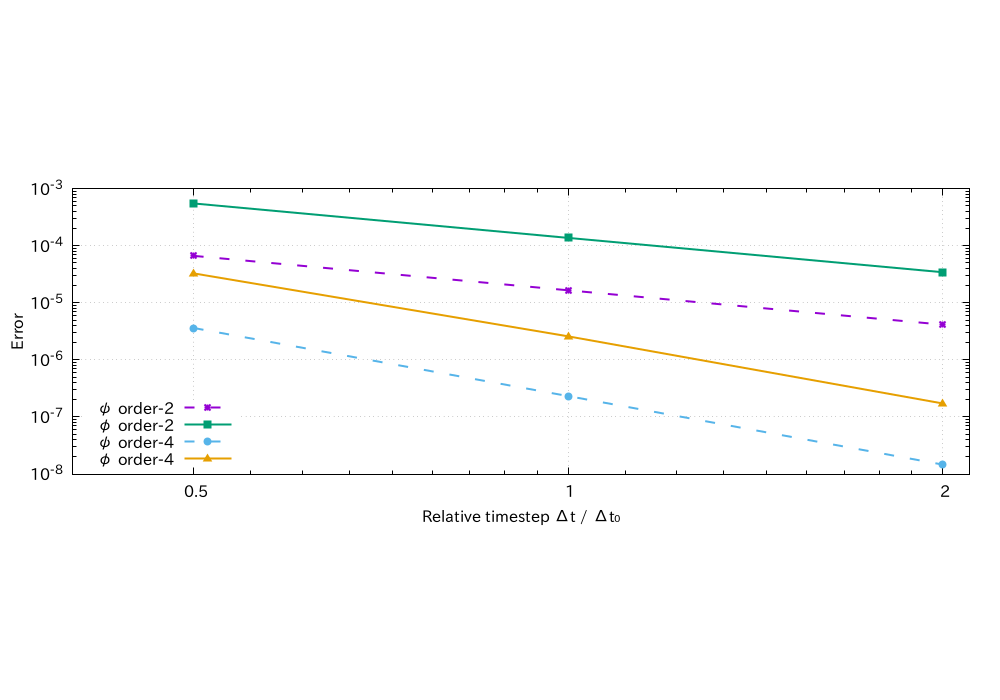
\includegraphics[scale=.18, trim={6 170 10 170},clip]{data/conv_compare.png} \\
% \end{figure}
%\input{tables/midpoint_zrp_p_richardson_realrun.tab}
%%\input{tables/simpson4_zrp_p_richardson_realrun.tab}
%\end{minipage}
%}
%\end{textblock*}
%
%\begin{textblock*}{0.5\linewidth}(0pt,190pt)
%\rotatebox{0}{
%\begin{minipage}{\linewidth}
%\Tiny
%\raggedright
%\input{tables/simpson4_zrp_p_richardson_realrun.tab}
%\end{minipage}
%}
%\end{textblock*}
%
%
%
%\begin{textblock*}{250pt}(220pt,80pt)
%\rotatebox{0}{
%\begin{minipage}{\linewidth}
%{
%\scriptsize
%\centering
%%	Left, From up to down $\rm {nsteps} = 10k,\, 15k,\, 20k$\\
%%	Up  $\rm {Np}=20, \rm{Ns}=100\; \rm{xmax}=2000$
%       \begin{align}
%       E \sim C (\Delta t)^p\nonumber \\
%       \log E = \log C + p\log (\Delta t) \nonumber\\
%        C_2 \sim 1.66(-5)   \nonumber \\
%        C_4 \sim 2.31(-7) \nonumber
%       \end{align}
%	\begin{align}
%%              \log E = \log C + p\log (\Delta t)  &\nonumber\\\vspace{20pt}
%		\rm{Np} = 20,\;\;\;\rm{Ns} = 100 \nonumber\\
%		\rm{xmax} \sim \rm{Np\,Ns}(1+1/4) /2 \nonumber\\
%		\omega_0 = 0.114\,{\rm a.u}\nonumber\\
%		F_0 = 0.03\,{\rm a.u}, \;\;T=5\tau\nonumber\\
%		{\rm nsteps} = 20 000,\, \;\;\Delta t_0=0.0689\nonumber
%	\end{align}
%%	\textcolor{red}{\textbf{The nonconvergence come from the fact that}
%%	$\rm{xmax}\sim \rm{Np\,Ns}$ here}
%
%}
%\end{minipage}
%}
%\end{textblock*}
%
%\begin{textblock*}{200pt}(250pt,220pt)
%	\begin{align}
%	p_k^{\rm self} & = \left({\rm err}_{k-1}/{\rm err}_{k}\right)/\log(2) \nonumber
%	\end{align}
%
%\end{textblock*}
%
%
%\end{frame}

